\documentclass{report}
\usepackage[utf8]{inputenc}
\usepackage{amsmath}
\usepackage{amsfonts}
\usepackage{hyperref}
\usepackage{tcolorbox}
\usepackage{breqn}
\usepackage{adjustbox}
\usepackage{changepage}
\usepackage{rotating}
\usepackage{algorithm}
\usepackage{algpseudocode}
\usepackage{ntheorem}
\usepackage[table,xcdraw]{xcolor}
\usepackage{longtable}
\usepackage{listings}

% Definition
\newtheorem{definition}{Definition}{\bfseries}{\itshape}
\newtheorem*{definition*}{Definition}{\bfseries}{\itshape}

% Theorem
\newtheorem{theorem}{Theorem}{\bfseries}{\itshape}

% Concept
\newtheorem*{concept}{}{\bfseries}{\itshape}

\title{Obtaining Linear Approximation Tables of AES and DES}
\author{Ana Clara Zoppi Serpa\\ Prof. Dr. Ricardo Dahab \\ Dr. Jorge Nakahara Jr.}
\date{\today}

\begin{document}

\maketitle

\tableofcontents

\chapter{Obtaining Linear Approximation Tables of AES and DES}

Linear Cryptanalysis (LC) was invented by Matsui \cite{Matsui1993LinearCM}. He describes how to apply it to the DES \cite{DES-FIPS} cipher, showing it is capable of breaking 8-round DES with $2^{21}$ known-plaintexts and 16-round DES with $2^{47}$ known-plaintexts. LAT -- Linear Approximation Tables --- of each DES $S$-Box are a core component for the attack. In this chapter, we focus on discussing how to obtain LATs for DES and AES \cite{AES-FIPS} and on exposing preliminary concepts related to LC.

We assume the reader is familiar with:
\begin{itemize}
    \item The DES cipher structure, available in \textcolor{red}{Chapter X}
    \item The AES cipher structure, available in \textcolor{red}{Chapter X}
    \item The Differential Cryptanalysis, DDTs and joint DDTs overview, available in \textcolor{red}{Chapter X}
\end{itemize}

\section{Notation}
\begin{itemize}
    \item $X_i$: a random variable
    \item $p_i$: the probability of $X_i$ being equal to $0$ ($Pr[X_i = 0]$)
    \item $\epsilon_i$: bias of a random variable $X_i$
    \item $\pi_S$: an hypothetical $S$-Box
    \item $n$: input size of an $S$-Box
    \item $m$: output size of an $S$-Box
    \item $X = (x_1, ..., x_n)$: $n$-tuple containing the inputs of $\pi_S$
    \item $Y = (y_1, ..., y_m)$: $m$-tuple containing the outputs of $\pi_s$
    \item $K$: cipher key
    \item $\gamma, \alpha, \beta$: bit masks
    \item $X \cdot \gamma$: dot product of $X$ and $\gamma$, i.e application of the bit mask $\gamma$ to the variable $X$
\end{itemize}

\section{Acronyms}
\begin{itemize}
    \item DES: Data Encryption Standard
    \item AES: Advanced Encryption Standard
    \item LC: Linear Cryptanalysis
    \item DC: Differential Cryptanalysis
    \item DDT: Difference Distribution Table
    \item LAT: Linear Approximation Table
\end{itemize}

\section{Preliminaries}

\subsection{Linear Cryptanalysis overview}

The goal of an LC attack is to find a probabilistic linear relationship between a subset of plaintext bits and a subset of state bits that immediately precede the substitutions performed in the last round of the cipher. In other words, \emph{the attacker seeks a subset of bits whose XOR behaves non-randomly}, i.e, taking value 0 with probability bounded away from $\frac{1}{2}$.

Assuming the attacker has a large number of plaintext and ciphertext pairs, all encrypted with the same key $K$, the attack works by decrypting each ciphertext, using all possible candidate keys for the last round of the iterated cipher. For each of these candidate keys, if there is a probabilistic linear relationship as aforementioned, the candidate key's counter is incremented by 1. At the end of the process, the correct key should have a frequency count which allows us to distinguish it from the other candidates.

Let $X_1, X_2, ...$ be independent random values taking on values from $\{0,1\}$, and $p_1, p_2, ...$ be the probabilities of each of them being equal to zero, i.e, $Pr[X_1 = 0] = p_1, Pr[X_2 = 0] = p_2$ and so forth. 
\begin{concept}[Bias \cite{Matsui1993LinearCM}]
The \emph{bias} of a random variable taking on the values $0$ and $1$ is defined as $\epsilon_i = p_i - \frac{1}{2}$. Consequently, $-1/2 \leq \epsilon_i \leq 1/2$, since $0 \leq p_i \leq 1$.
\end{concept}

\begin{concept}[Piling-Up Lemma \cite{Matsui1993LinearCM}]
The bias of a random variable $X_{i_1} \oplus X_{i_2} \oplus ... \oplus X_{i_k}$ is $\epsilon_{i_1, i_2, ..., i_k} = 2^{k-1} \prod_{j=1}^{k} \epsilon_{i_j}$.
\end{concept}

The Linear Cryptanalysis attack exploits sums of random variables, e.g $S$-boxes inputs and outputs, their biases, and, extending the concept to the whole iterated cipher, extracts the key. 

Considering an example $S$-box $\pi_S : \{0,1\}^n \rightarrow \{0,1\}^m$, if an input $n$-tuple $X = (x_1, ..., x_n)$ is chosen randomly, each coordinate $x_i$ is a random variable $X_i$ taking values from $\{0,1 \}$. These variables are independent. A randomly chosen output tuple $Y = (y_1, ..., y_m)$, similarly, defines a random variable $Y_j$, also taking values from $\{0,1 \}$. However, they are not necessarily independent on each other, nor they are independent of the $X_i$ variables.

%If $(y_1, ..., y_m) \neq \pi_s(x_1, ..., x_n)$ then 

%$$Pr[X_1 = x_1, ..., X_n = x_n, Y_1 = y_1, ..., Y_m = y_m] = 0.$$ 

%However, if $(y_1, ..., y_m) = \pi_s(x_1, ..., x_n)$, then 

%$$Pr[X_1 = x_1, ..., X_n = x_n, Y_1 = y_1, ..., Y_m = y_m] = 2^{-n},$$ 

%since $$Pr[X_1 = x_1, ..., X_n = x_n] = 2^{-n}$$

%and $$Pr[Y_1 = y_1, ..., Y_m = y_m | X_1 = x_1, ..., X_n = x_n] = 1.$$

It is possible to compute the bias of a random variable of the form $X_{i_1} \oplus ... \oplus X_{i_z} \oplus Y_{j_1} \oplus ... \oplus Y_{j_l}$, from the Piling-up Lemma. When such bias is bounded away from $\frac{1}{2}$, a Linear Cryptanalysis attack can be mounted, if the amount of required plaintexts for the attack (which is inversely proportional to the bias) does not surpass the cipher's codebook, i.e if the final bias value is not too small.

\subsection{Bit masks and Linear Approximation Tables}

\begin{concept}[Bit mask \cite{Matsui1993LinearCM}]
A bit mask $\gamma$ selects fixed specific bits of a variable $X$. For example, $\gamma = [i]$ refers to selecting only the $i$-th bit, $\gamma = [i, j, k]$ refers to selecting the $i$-th, $j$-th and $k$-th bits, and so forth, and XORing them. Formally, the result of the mask selection for a variable $X$ can be obtained by means of the \emph{dot product} $X \cdot \gamma$.
\end{concept}

For example, let $X = 1111_2$ and $\gamma = [1, 2] = 0110_2$. Then

$$X \cdot \gamma = (0\cdot1) \oplus (1\cdot1) \oplus (1\cdot1) \oplus (0\cdot1) = 0_2,$$

because $\gamma$ selects bits $1$ and $2$, considering that the starting bit, $0$, is the least significant bit, and XORs them. Bits 0 and 3 are not selected. Bit masks are used by Matsui \cite{Matsui1993LinearCM} to represent linear relationships (or approximations) between subsets of bits of the cipher. As another example, we show the usage of bit masks to represent linear relationship in the logical XOR of two variables.

Let $A = (..., a_1, a_0)$, $B = (..., b_1, b_0)$ and $C = A \oplus B$. Each $i$-th bit of $C$ depends linearly (and individually) on the $i$-th bits of $A$ and $B$, due to the bitwise XOR. In other words, $c_i = a_i \oplus b_i$. Equivalently, using bit mask notation, $C \cdot \gamma = A \cdot \gamma \oplus B \cdot \gamma$, with $\gamma = [i]$. Note that, when dealing with bit masks, we have switched the indexing of bits: we start from left to right, instead of from right to left. Also, the bit indices start at 0. We do this to follow the notation presented by Matsui \cite{Matsui1993LinearCM}.

\begin{concept}[Linear Approximation Table of an $S$-Box]
For an $n$-bit input $S$-Box $S$, the LAT of $S$ is the table $\mathcal{L}$ such that  $\mathcal{L}[\alpha][\beta] = \# \{ x \in \mathbb{Z}_2^n : \alpha \cdot x = \beta \cdot S(x)\} - 2^{n-1}$, where $\alpha$ and $\beta$ are masks. In other words, a LAT entry $[\alpha, \beta]$ counts how far the parity of $\alpha \cdot x \oplus \beta \cdot S(x)$ deviates (or not) from $2^{n-1}$.
\end{concept}

\begin{concept}[Trivial and non-trivial linear relations]
A trivial linear relation possesses bias equal to zero. A non-trivial linear relation possesses non-zero bias. In Linear Cryptanalysis, we seek non-trivial linear relations.
\end{concept}

\begin{concept}[Trivial and non-trivial masks]
We say that $\alpha = 0$ is a trivial mask, whilst $\alpha \neq 0$ is a non-trivial mask. In LC, we are interested in LAT entries with non-trivial input masks.
\end{concept}

Each entry $\mathcal{L}[\alpha][\beta]$ indicates whether there is a non-trivial linear relation between $\alpha$ input bits and $\beta$ output bits of $S$.

\begin{concept}[Linear Uniformity]
The linear uniformity of an $S$-Box is 

$$\gamma_{max} = max_{\alpha\not= 0} |LAT(\alpha,\beta)|,$$ 
where $|x|$ denotes the absolute value of $x$. It shows the largest entry in the LAT of a given $S$-Box.
\end{concept}

\section{Computing a LAT}

Let $S$ be an $n$-bit input and $m$-bit output $S$-Box. In order to obtain its LAT $\mathcal{L}$, Algorithm \ref{alg:get-lat} can be used. $2^{n} \times 2^{m} \times 2^{n}$ $S$-Box lookups are necessary, and $2 \times 2^{n} \times 2^{m} \times 2^{n}$ mask selection steps. Therefore, the computational complexity is $O(2^{2n + m})$ $S$-Box lookups, considering $S$-Box lookups and mask selection operations to be constant time.

For a DES $S$-Box, $n = 6$ and $m = 4$, resulting in $2^{16}$ run time complexity. For an AES $S$-Box, $n = m = 8$, resulting in $2^{24}$ complexity. In the case of AES and DES, since we are dealing with integer values, the mask selection can be performed with logical AND, XOR and bit shift operators.

\begin{algorithm}[H]
\caption{Obtaining the LAT of an $S$-box}
\label{alg:get-lat}
\begin{algorithmic}[1]
    \State Initialize $\mathcal{L}$ with $2^{n-1}$ (the bias) in all entries
    \For{$\alpha = 0, ..., 2^n - 1$}
        \For{$\beta = 0, ..., 2^m - 1$}
            \For {$x = 0, ..., 2^n - 1$}
                \State $l \gets \alpha \cdot x$ \Comment{Select bits according to the input mask}
                \State $r \gets \beta \cdot S(x)$ \Comment{Select bits according to the output mask}
                \If {$l = r$}
                    \State $\mathcal{L}[\alpha][\beta] \gets \mathcal{L}[\alpha][\beta] + 1$
                \EndIf
            \EndFor
        \EndFor
    \EndFor
\State \textbf{return} $\mathcal{L}$
\end{algorithmic}
\end{algorithm}

It is also possible to compute LATs using the Walsh-Hadamard Transform of a Boolean Function, as explained in \cite{Anne2016}.

\subsection{Practical run time remarks}
In a personal computer with a 2.6 GHz Intel Core i7 6-Core processor, a LAT for a DES $S$-Box could be obtained in less than 2 seconds, and a LAT for one AES $S$-Box could be obtained in less than 2 minutes.

\section{LATs for DES}

Table \ref{tbl:lu-des} shows the linear uniformitiy of each DES $S$-Box. Note that $S_5$ presents the largest linear uniformity, which signals it contains the most effective linear relationship to be exploited in an LC attack. For this reason, Matsui \cite{Matsui1993LinearCM} exploits $S_5$ to mount his attack.
Tables \ref{tbl:lat1} to \ref{tbl:lat8} show the LATs for $S$-Boxes $S_1$ to $S_8$, respectively. They are also available as \texttt{.csv} files at \textcolor{red}{Git link}, together with the code used to obtain them.

\begin{table}[H]
\centering
\begin{tabular}{|l|l|l|l|l|l|l|l|l|}
\hline
$S$-Box           & $S_1$ & $S_2$ & $S_3$ & $S_4$ & $S_5$ & $S_6$ & $S_7$ & $S_8$ \\ \hline
Linear uniformity & 18    & 16    & 16    & 16    & 20    & 14    & 18    & 16    \\ \hline
\end{tabular}
\caption{Linear Uniformities of each DES $S$-Box}
\label{tbl:lu-des}
\end{table}

% Please add the following required packages to your document preamble:
% \usepackage{longtable}
% Note: It may be necessary to compile the document several times to get a multi-page table to line up properly
\begin{longtable}[c]{|l|l|l|l|l|l|l|l|l|l|l|l|l|l|l|l|l|}
\hline
            & \textbf{0} & \textbf{1} & \textbf{2} & \textbf{3} & \textbf{4} & \textbf{5} & \textbf{6} & \textbf{7} & \textbf{8} & \textbf{9} & \textbf{10} & \textbf{11} & \textbf{12} & \textbf{13} & \textbf{14} & \textbf{15}  \\ \hline
\endfirsthead
%
\endhead
%
\textbf{0}  & 32         & 0          & 0          & 0          & 0          & 0          & 0          & 0          & 0          & 0          & 0           & 0           & 0           & 0           & 0           & 0            \\ \hline
\textbf{1}  & 0          & 0          & 0          & 0          & 0          & 0          & 0          & 0          & 0          & 0          & 0           & 0           & 0           & 0           & 0           & 0            \\ \hline
\textbf{2}  & 0          & -2         & -2         & -4         & -2         & 0          & -4         & 6          & 2          & 0          & 0           & 6           & 4           & -2          & -6          & 4            \\ \hline
\textbf{3}  & 0          & -2         & -2         & -4         & -2         & 0          & -4         & 6          & 2          & 8          & 0           & -2          & 4           & 6           & -6          & -4           \\ \hline
\textbf{4}  & 0          & 2          & -2         & -4         & -2         & 0          & -4         & -6         & -2         & 4          & 8           & 2           & 0           & -2          & -6          & 12           \\ \hline
\textbf{5}  & 0          & -2         & -2         & 0          & -2         & -4         & -4         & -2         & 2          & -4         & -4          & 2           & 4           & -10         & -2          & -4           \\ \hline
\textbf{6}  & 0          & 0          & 0          & 4          & 0          & 4          & 0          & 0          & 0          & -4         & 4           & 4           & 0           & 0           & -4          & -8           \\ \hline
\textbf{7}  & 0          & -4         & 0          & 8          & 0          & 0          & 0          & 4          & 4          & -4         & -8          & -4          & 4           & 0           & 0           & 0            \\ \hline
\textbf{8}  & 0          & 4          & -2         & 6          & -6         & -6         & 0          & -4         & -4         & -4         & 2           & -2          & 2           & -2          & 0           & 0            \\ \hline
\textbf{9}  & 0          & 0          & 6          & -6         & -2         & -6         & 4          & -4         & 0          & -4         & -2          & 6           & 2           & -6          & 0           & -4           \\ \hline
\textbf{10} & 0          & -2         & 0          & 2          & 0          & 6          & 8          & 2          & -2         & 0          & -2          & 4           & -2          & 0           & -2          & 4            \\ \hline
\textbf{11} & 0          & 2          & -8         & -2         & -4         & -10        & 4          & 2          & -6         & 8          & 2           & 4           & -2          & -4          & -2          & 0            \\ \hline
\textbf{12} & 0          & -2         & 0          & 6          & 0          & 2          & 0          & 2          & 2          & 0          & 6           & -4          & 2           & -4          & 6           & 0            \\ \hline
\textbf{13} & 0          & 6          & 0          & 6          & 4          & -2         & -4         & -2         & 2          & 0          & 6           & 4           & -2          & 8           & -6          & -4           \\ \hline
\textbf{14} & 0          & 0          & -2         & -2         & 2          & 2          & 0          & 0          & 4          & 4          & 6           & -2          & 2           & 2           & -4          & 4            \\ \hline
\textbf{15} & 0          & 0          & -2         & 6          & -2         & -2         & 4          & -4         & -4         & -4         & -2          & -2          & -2          & -2          & 0           & 0            \\ \hline
\textbf{16} & 0          & 2          & 2          & 0          & -2         & 0          & 4          & -6         & 0          & 6          & 2           & -4          & 6           & -4          & -4          & \textbf{-18} \\ \hline
\textbf{17} & 0          & 2          & -2         & -4         & 2          & -4         & -4         & 10         & -4         & 2          & 2           & -4          & -2          & -4          & 0           & -6           \\ \hline
\textbf{18} & 0          & 4          & 0          & 0          & -4         & 4          & 0          & 4          & -6         & 2          & 2           & 6           & 2           & 6           & 6           & -10          \\ \hline
\textbf{19} & 0          & 4          & -4         & -4         & 0          & 0          & -8         & -12        & -2         & -2         & -6          & 6           & 2           & 6           & 2           & 2            \\ \hline
\textbf{20} & 0          & 4          & 0          & 4          & -8         & -4         & 4          & 0          & 2          & 6          & -2          & 2           & 6           & 2           & -2          & 2            \\ \hline
\textbf{21} & 0          & 0          & 4          & -4         & -4         & 4          & 4          & -4         & 10         & 2          & 2           & 2           & -6          & 2           & 6           & -2           \\ \hline
\textbf{22} & 0          & 6          & 2          & 0          & 2          & -4         & 0          & 2          & 4          & 2          & 2           & 0           & -2          & 0           & 0           & 2            \\ \hline
\textbf{23} & 0          & 2          & 6          & -8         & 6          & 4          & 0          & -2         & -12        & -2         & -2          & 0           & -6          & 0           & 0           & -2           \\ \hline
\textbf{24} & 0          & 2          & 8          & 2          & 0          & 6          & 4          & 2          & 4          & -2         & 4           & 6           & 0           & -2          & -4          & 2            \\ \hline
\textbf{25} & 0          & -2         & 4          & -6         & 0          & -6         & 0          & 2          & 4          & -6         & 8           & 6           & 0           & 2           & 0           & -6           \\ \hline
\textbf{26} & 0          & 0          & -6         & 2          & -2         & -2         & 4          & 4          & -2         & -2         & 0           & 0           & -4          & 4           & 2           & 2            \\ \hline
\textbf{27} & 0          & 4          & 6          & 2          & -10        & 2          & -8         & 4          & -2         & -6         & 4           & 0           & 4           & 0           & -2          & 2            \\ \hline
\textbf{28} & 0          & -4         & 2          & 2          & 2          & -6         & 0          & -4         & -2         & -2         & 4           & 0           & 0           & 4           & 2           & 2            \\ \hline
\textbf{29} & 0          & 4          & -2         & -2         & 2          & -6         & -4         & 0          & 2          & 2          & -4          & 0           & -12         & 0           & -6          & -6           \\ \hline
\textbf{30} & 0          & 2          & 0          & -2         & 4          & -2         & 0          & -2         & 0          & 6          & -4          & -2          & 0           & -2          & 0           & 2            \\ \hline
\textbf{31} & 0          & 2          & -4         & 2          & -4         & -2         & 4          & 2          & 4          & -6         & 4           & -2          & -4          & 2           & 0           & 2            \\ \hline
\textbf{32} & 0          & 0          & 0          & 0          & 0          & 0          & 0          & 0          & 0          & 0          & 0           & 0           & 0           & 0           & 0           & 0            \\ \hline
\textbf{33} & 0          & 0          & 0          & 0          & 0          & 0          & 0          & 0          & 0          & 0          & 0           & 0           & 0           & 0           & 0           & 0            \\ \hline
\textbf{34} & 0          & 2          & -2         & 0          & 2          & 0          & 0          & 6          & -2         & 0          & -4          & 6           & 4           & 10          & 10          & 0            \\ \hline
\textbf{35} & 0          & 2          & -2         & 0          & 2          & 0          & 0          & 6          & 6          & 0          & 4           & -10         & -4          & -6          & 2           & 0            \\ \hline
\textbf{36} & 0          & 2          & -6         & -8         & 2          & 4          & 4          & 2          & 2          & 0          & 0           & 2           & 0           & 6           & -10         & 0            \\ \hline
\textbf{37} & 0          & -2         & 2          & 4          & 2          & 0          & -4         & -2         & -2         & 0          & 4           & 2           & -4          & 6           & -6          & 0            \\ \hline
\textbf{38} & 0          & 4          & 4          & -4         & 8          & -8         & 4          & 0          & 0          & -8         & 0           & -4          & 0           & 4           & 0           & 0            \\ \hline
\textbf{39} & 0          & 0          & -4         & -8         & -8         & 4          & -4         & -4         & 4          & -8         & -4          & -4          & 4           & 4           & -4          & 0            \\ \hline
\textbf{40} & 0          & 4          & -2         & -2         & -2         & -2         & -4         & 0          & 4          & 4          & 2           & 6           & -2          & -6          & 12          & 4            \\ \hline
\textbf{41} & 0          & 0          & -2         & -6         & 2          & -2         & -8         & 8          & 0          & -4         & -2          & -2          & 6           & -2          & -4          & 0            \\ \hline
\textbf{42} & 0          & 2          & 0          & -2         & 0          & 2          & 0          & -2         & 2          & -8         & -6          & -4          & 2           & 0           & 2           & -4           \\ \hline
\textbf{43} & 0          & -10        & 0          & 2          & -4         & 2          & 4          & 6          & -2         & 0          & -10         & 4           & 2           & -4          & -6          & 0            \\ \hline
\textbf{44} & 0          & 6          & -4         & 2          & 8          & 2          & 4          & 6          & -2         & -4         & -2          & 12          & -2          & -8          & -2          & 0            \\ \hline
\textbf{45} & 0          & -2         & -4         & 2          & -4         & -2         & 0          & 2          & -2         & -4         & -2          & 4           & -6          & 4           & 2           & -4           \\ \hline
\textbf{46} & 0          & -4         & 2          & 6          & 6          & -6         & -8         & 4          & -4         & 0          & 2           & 6           & 6           & 2           & 4           & 0            \\ \hline
\textbf{47} & 0          & -4         & 2          & -2         & 2          & -10        & 12         & 0          & -4         & 0          & 2           & -2          & 10          & 6           & 0           & 4            \\ \hline
\textbf{48} & 0          & -2         & -2         & 0          & -2         & 4          & 0          & 2          & 0          & 2          & 6           & 4           & 6           & 0           & 0           & -2           \\ \hline
\textbf{49} & 0          & -2         & 2          & 4          & 2          & 0          & 0          & -6         & -4         & -2         & -2          & -4          & -2          & 0           & -4          & 2            \\ \hline
\textbf{50} & 0          & -4         & -4         & -4         & 0          & 0          & 0          & 4          & -2         & -2         & -6          & -2          & -6          & 6           & 2           & 2            \\ \hline
\textbf{51} & 0          & -4         & 0          & 0          & 4          & -4         & 0          & -4         & -6         & 2          & 2           & -2          & 2           & -2          & -2          & -2           \\ \hline
\textbf{52} & 0          & 8          & -8         & 8          & 4          & 4          & 0          & 0          & -2         & -2         & 2           & -6          & 6           & 6           & -2          & -2           \\ \hline
\textbf{53} & 0          & 4          & -4         & 0          & -8         & -4         & 0          & -4         & -2         & 2          & -2          & 2           & 2           & -2          & -2          & 2            \\ \hline
\textbf{54} & 0          & 6          & 2          & -8         & 2          & -4         & 8          & 2          & 4          & -6         & 2           & 0           & 6           & 0           & 0           & 2            \\ \hline
\textbf{55} & 0          & 2          & -10        & 0          & 6          & 4          & 8          & -2         & 4          & 6          & -2          & 0           & 2           & 0           & 0           & -2           \\ \hline
\textbf{56} & 0          & -10        & 4          & 2          & -4         & -2         & 4          & -2         & 4          & 2          & 0           & 6           & -4          & 6           & -4          & -2           \\ \hline
\textbf{57} & 0          & 2          & 0          & -6         & -4         & 2          & 0          & -2         & -4         & 6          & -4          & -2          & 4           & 2           & 8           & -2           \\ \hline
\textbf{58} & 0          & 0          & 6          & -2         & 6          & 6          & 0          & 0          & 2          & 2          & 0           & 0           & 8           & 0           & 2           & 2            \\ \hline
\textbf{59} & 0          & 4          & 2          & -2         & -2         & 10         & 4          & 0          & -14        & -2         & 4           & 0           & 0           & -4          & -2          & 2            \\ \hline
\textbf{60} & 0          & 0          & 10         & -2         & -6         & -2         & 0          & 8          & -6         & 6          & 0           & -8          & -4          & 4           & -2          & 2            \\ \hline
\textbf{61} & 0          & 8          & -2         & 2          & -6         & -2         & 4          & 4          & -2         & -6         & 0           & 0           & 0           & 0           & -2          & 2            \\ \hline
\textbf{62} & 0          & 2          & 0          & -2         & -8         & 2          & 4          & 2          & 0          & -2         & 4           & -2          & -4          & 2           & 4           & -2           \\ \hline
\textbf{63} & 0          & -14        & -12        & -6         & 0          & 2          & 0          & -2         & -4         & -6         & 12          & -2          & 0           & -2          & 4           & -2           \\ \hline
\caption{LAT for $S_1$ of DES}
\label{tbl:lat1}
\end{longtable}
% Please add the following required packages to your document preamble:
% \usepackage{longtable}
% Note: It may be necessary to compile the document several times to get a multi-page table to line up properly
\begin{longtable}[c]{|l|l|l|l|l|l|l|l|l|l|l|l|l|l|l|l|l|}
\hline
            & \textbf{0} & \textbf{1} & \textbf{2} & \textbf{3} & \textbf{4} & \textbf{5} & \textbf{6} & \textbf{7} & \textbf{8} & \textbf{9} & \textbf{10} & \textbf{11}  & \textbf{12} & \textbf{13} & \textbf{14} & \textbf{15}  \\ \hline
\endfirsthead
%
\endhead
%
\textbf{0}  & 32         & 0          & 0          & 0          & 0          & 0          & 0          & 0          & 0          & 0          & 0           & 0            & 0           & 0           & 0           & 0            \\ \hline
\textbf{1}  & 0          & 0          & 0          & 0          & 0          & 0          & 0          & 0          & 0          & 0          & 0           & 0            & 0           & 0           & 0           & 0            \\ \hline
\textbf{2}  & 0          & 0          & 0          & 4          & 0          & 0          & -4         & 0          & 0          & 0          & -4          & 0            & 0           & 0           & 0           & 4            \\ \hline
\textbf{3}  & 0          & 0          & 4          & -8         & 0          & 8          & 0          & -4         & 0          & 0          & -8          & -4           & 0           & 8           & -4          & 8            \\ \hline
\textbf{4}  & 0          & -2         & 2          & 4          & 2          & 0          & 4          & 6          & 0          & 6          & -2          & 0            & 2           & 0           & 0           & 10           \\ \hline
\textbf{5}  & 0          & 2          & 2          & 0          & 2          & -4         & 4          & -6         & 0          & -6         & 6           & 4            & -6          & 4           & 0           & -2           \\ \hline
\textbf{6}  & 0          & -2         & -2         & -4         & -2         & -4         & 0          & -2         & -4         & 2          & 2           & 0            & 2           & 0           & 4           & 10           \\ \hline
\textbf{7}  & 0          & 2          & 2          & -4         & -2         & 0          & 4          & -2         & -4         & 6          & 6           & 0            & -6          & -4          & 0           & 2            \\ \hline
\textbf{8}  & 0          & 0          & 2          & 2          & -2         & 2          & 4          & 0          & -2         & -6         & -4          & 0            & 0           & 0           & 10          & -6           \\ \hline
\textbf{9}  & 0          & 0          & -2         & -2         & -2         & 2          & 8          & 4          & -2         & 2          & 0           & -4           & 0           & 8           & -10         & -2           \\ \hline
\textbf{10} & 0          & -4         & 2          & 2          & 2          & 2          & -4         & -8         & 2          & 2          & 4           & 0            & 0           & 4           & -6          & 2            \\ \hline
\textbf{11} & 0          & 4          & 2          & 10         & 2          & 2          & 4          & 0          & 2          & 2          & 4           & 0            & 0           & -4          & 2           & 2            \\ \hline
\textbf{12} & 0          & -2         & 4          & -2         & 0          & 2          & 0          & 6          & -2         & 0          & 2           & 0            & 2           & 0           & -6          & -4           \\ \hline
\textbf{13} & 0          & -6         & 0          & -2         & 0          & 6          & 4          & -10        & 6          & -4         & 6           & 0            & 2           & -4          & -2          & 4            \\ \hline
\textbf{14} & 0          & -6         & 0          & 2          & 0          & -2         & -8         & 6          & -2         & 4          & 2           & 0            & 2           & 4           & -2          & 0            \\ \hline
\textbf{15} & 0          & -2         & 0          & -2         & 0          & 2          & 0          & 10         & 6          & 8          & 2           & 4            & 2           & 0           & -2          & 4            \\ \hline
\textbf{16} & 0          & 0          & -4         & 4          & 0          & 0          & 0          & 0          & 0          & 0          & 4           & 4            & 4           & -12         & -4          & -12 \\ \hline
\textbf{17} & 0          & 0          & 0          & 0          & 0          & -8         & 4          & 4          & 0          & 0          & 8           & 0            & -4          & 4           & 8           & 0            \\ \hline
\textbf{18} & 0          & 0          & 0          & 4          & 0          & 8          & 0          & 4          & 0          & 0          & -4          & 8            & -4          & -12         & 0           & 12           \\ \hline
\textbf{19} & 0          & 0          & -8         & 4          & 0          & 8          & 8          & 4          & 0          & 0          & -4          & 0            & 4           & -4          & 8           & -4           \\ \hline
\textbf{20} & 0          & -2         & -6         & -4         & -2         & 4          & -4         & -2         & -4         & 2          & 2           & -4           & 6           & -4          & 0           & 2            \\ \hline
\textbf{21} & 0          & 10         & -2         & -4         & -2         & 0          & 0          & -2         & 4          & 6          & 6           & -4           & -2          & 0           & 4           & 2            \\ \hline
\textbf{22} & 0          & -2         & -6         & 0          & 2          & 0          & 4          & 2          & 8          & -2         & 2           & 0            & 6           & 4           & 0           & -2           \\ \hline
\textbf{23} & 0          & 10         & 2          & 4          & 2          & 4          & -4         & -2         & 0          & 2          & 2           & -4           & -2          & 0           & 0           & 2            \\ \hline
\textbf{24} & 0          & -4         & 2          & -2         & 2          & 2          & 4          & 4          & -2         & -2         & 4           & 4            & 0           & 4           & -2          & 2            \\ \hline
\textbf{25} & 0          & 4          & -6         & 6          & 2          & 2          & 4          & -4         & -2         & -2         & 4           & -4           & 8           & 4           & -2          & 2            \\ \hline
\textbf{26} & 0          & 8          & -2         & 2          & -2         & 2          & 0          & 0          & 2          & 6          & 0           & 0            & 0           & 0           & 2           & -2           \\ \hline
\textbf{27} & 0          & -8         & 10         & 6          & -2         & 2          & 4          & -4         & 2          & -2         & -4          & -4           & -8          & 0           & -2          & -6           \\ \hline
\textbf{28} & 0          & 2          & 8          & -2         & 0          & -2         & 0          & 2          & 2          & 0          & -6          & 4            & 10          & -4          & 2           & 0            \\ \hline
\textbf{29} & 0          & -2         & 0          & 2          & 0          & -6         & 0          & -2         & 2          & 4          & 2           & 0            & 10          & 0           & 2           & 4            \\ \hline
\textbf{30} & 0          & -2         & 0          & 6          & 0          & 2          & 4          & -2         & 2          & 4          & -2          & 0            & 2           & 0           & 2           & 0            \\ \hline
\textbf{31} & 0          & 2          & -4         & 6          & 0          & -2         & -8         & -2         & -14        & 0          & 2           & 0            & 2           & 4           & -2          & 0            \\ \hline
\textbf{32} & 0          & 0          & 0          & 0          & 0          & 0          & 0          & 0          & 0          & 0          & 0           & 0            & 0           & 0           & 0           & 0            \\ \hline
\textbf{33} & 0          & 0          & 0          & 0          & 0          & 0          & 0          & 0          & 0          & 0          & 0           & 0            & 0           & 0           & 0           & 0            \\ \hline
\textbf{34} & 0          & 0          & 0          & 4          & 0          & -8         & 4          & 0          & 0          & 0          & -4          & \textbf{-16} & 0           & -8          & -8          & 4            \\ \hline
\textbf{35} & 0          & 0          & -4         & 0          & 0          & 0          & 0          & 4          & 0          & 0          & 0           & 4            & 0           & 0           & -4          & 0            \\ \hline
\textbf{36} & 0          & -2         & -2         & 0          & -2         & -4         & 4          & -10        & 0          & 6          & -6          & -4           & 6           & 4           & 8           & 2            \\ \hline
\textbf{37} & 0          & -6         & -2         & 4          & -2         & 0          & 4          & 2          & 0          & 2          & 2           & -8           & -2          & 0           & 8           & -2           \\ \hline
\textbf{38} & 0          & 6          & -6         & 0          & -14        & 0          & 0          & -2         & -4         & -6         & -2          & 4            & -2          & -4          & -4          & 2            \\ \hline
\textbf{39} & 0          & 2          & 6          & 0          & 2          & -4         & -4         & -2         & -4         & 6          & -6          & 4            & 6           & 0           & 0           & -6           \\ \hline
\textbf{40} & 0          & -4         & 2          & -2         & 2          & 2          & 0          & -8         & 2          & 2          & 0           & 8            & 8           & -4          & -6          & -2           \\ \hline
\textbf{41} & 0          & -4         & -2         & -6         & 2          & 2          & 4          & -4         & -6         & 2          & -4          & -4           & 0           & -4          & -2          & -6           \\ \hline
\textbf{42} & 0          & 8          & 2          & -2         & 6          & -6         & 0          & 0          & -2         & 2          & 0           & 0            & 0           & 0           & -6          & -2           \\ \hline
\textbf{43} & 0          & 0          & -6         & -2         & 6          & 10         & 0          & 0          & -10        & 10         & 0           & 0            & -8          & 0           & 2           & -2           \\ \hline
\textbf{44} & 0          & -6         & 0          & 6          & 0          & -2         & -4         & -2         & 2          & -8         & 2           & 4            & -2          & 0           & 2           & 8            \\ \hline
\textbf{45} & 0          & -2         & -4         & -2         & 0          & -6         & 0          & -10        & 2          & 4          & -2          & 4            & -10         & -4          & -2          & 0            \\ \hline
\textbf{46} & 0          & -2         & -4         & 2          & 8          & 2          & 4          & -2         & -6         & -4         & -6          & 4            & -2          & 4           & -2          & 4            \\ \hline
\textbf{47} & 0          & -6         & 4          & -2         & -8         & -2         & 4          & 2          & -6         & 0          & 10          & 0            & 6           & 0           & -2          & 0            \\ \hline
\textbf{48} & 0          & 0          & -4         & 4          & -4         & -4         & 4          & 4          & 0          & 0          & -4          & -4           & 0           & 0           & -8          & 0            \\ \hline
\textbf{49} & 0          & 0          & 0          & 0          & 4          & -4         & 0          & 0          & 0          & 0          & 0           & -8           & 0           & -8          & -4          & 4            \\ \hline
\textbf{50} & 0          & 0          & 0          & 4          & 4          & 4          & 4          & 0          & 0          & 0          & 4           & 0            & 0           & 0           & -4          & 0            \\ \hline
\textbf{51} & 0          & 0          & 0          & -4         & -4         & -4         & -4         & 0          & 0          & 0          & -4          & 0            & 0           & 0           & 4           & 0            \\ \hline
\textbf{52} & 0          & -10        & -2         & -8         & 6          & 4          & -8         & 2          & 4          & 2          & 6           & -8           & -2          & -4          & 4           & -2           \\ \hline
\textbf{53} & 0          & -6         & 2          & 0          & -2         & 0          & 4          & 2          & -4         & -2         & -6          & 0            & -2          & 0           & 0           & -2           \\ \hline
\textbf{54} & 0          & -2         & -2         & 4          & -6         & 0          & 8          & -2         & 0          & 6          & 6           & 4            & -2          & 4           & -4          & 2            \\ \hline
\textbf{55} & 0          & 2          & -2         & -8         & -14        & 4          & 0          & 2          & 8          & 2          & -2          & 0            & -2          & 0           & -4          & -2           \\ \hline
\textbf{56} & 0          & 0          & 2          & 2          & -6         & -2         & -4         & 0          & 2          & -2         & 0           & -4           & -4          & -4          & 2           & 2            \\ \hline
\textbf{57} & 0          & 8          & 10         & -6         & 2          & 6          & 4          & 0          & -6         & -10        & 8           & -4           & 4           & -4          & 2           & 2            \\ \hline
\textbf{58} & 0          & -4         & -2         & 6          & -2         & -2         & -8         & 4          & -2         & -2         & 4           & 0            & -4          & 0           & -2          & -2           \\ \hline
\textbf{59} & 0          & -4         & 2          & 2          & -10        & 6          & -4         & 0          & -10        & -2         & 0           & -4           & 4           & 0           & 2           & 2            \\ \hline
\textbf{60} & 0          & -2         & -4         & -2         & 4          & -2         & 0          & -2         & -2         & 0          & 2           & 0            & 2           & -8          & -2          & 0            \\ \hline
\textbf{61} & 0          & 2          & 4          & 10         & -4         & 10         & -8         & -6         & 6          & 4          & 2           & -4           & 2           & 4           & -2          & -4           \\ \hline
\textbf{62} & 0          & 2          & -12        & -2         & 4          & 2          & -4         & 2          & 6          & -12        & -2          & -4           & 2           & 4           & -2          & 0            \\ \hline
\textbf{63} & 0          & -2         & -8         & -2         & -4         & -2         & 0          & -6         & -2         & 0          & 2           & 4            & 2           & 0           & 2           & 0            \\ \hline
\caption{LAT for $S_2$ of DES}
\label{tbl:lat2}
\end{longtable}
% Please add the following required packages to your document preamble:
% \usepackage{longtable}
% Note: It may be necessary to compile the document several times to get a multi-page table to line up properly
\begin{longtable}[c]{|l|l|l|l|l|l|l|l|l|l|l|l|l|l|l|l|l|}
\hline
            & \textbf{0} & \textbf{1} & \textbf{2} & \textbf{3} & \textbf{4} & \textbf{5} & \textbf{6} & \textbf{7} & \textbf{8} & \textbf{9} & \textbf{10} & \textbf{11} & \textbf{12} & \textbf{13} & \textbf{14} & \textbf{15} \\ \hline
\endfirsthead
%
\endhead
%
\textbf{0}  & 32         & 0          & 0          & 0          & 0          & 0          & 0          & 0          & 0          & 0          & 0           & 0           & 0           & 0           & 0           & 0           \\ \hline
\textbf{1}  & 0          & 0          & 0          & 0          & 0          & 0          & 0          & 0          & 0          & 0          & 0           & 0           & 0           & 0           & 0           & 0           \\ \hline
\textbf{2}  & 0          & 2          & -2         & -4         & 0          & -2         & -6         & 4          & 0          & 6          & -2          & -8          & 4           & -2          & -2          & -4          \\ \hline
\textbf{3}  & 0          & -2         & -2         & 0          & 4          & -2         & -2         & -4         & -4         & -2         & 2           & 0           & -4          & 2           & -2          & 0           \\ \hline
\textbf{4}  & 0          & -4         & 0          & 0          & 2          & -2         & -6         & 2          & 0          & 4          & 4           & -4          & -6          & -10         & 6           & -2          \\ \hline
\textbf{5}  & 0          & 0          & 0          & -4         & 2          & 2          & 2          & 6          & 0          & 0          & 4           & 0           & 2           & -6          & 6           & 2           \\ \hline
\textbf{6}  & 0          & -2         & 2          & 0          & 2          & -4         & 0          & 2          & 0          & -6         & -2          & 0           & -2          & 4           & 8           & -2          \\ \hline
\textbf{7}  & 0          & -2         & 2          & 0          & -2         & 8          & 4          & 6          & -4         & -2         & 2           & -4          & -10         & 4           & 0           & -2          \\ \hline
\textbf{8}  & 0          & 0          & 6          & -6         & 0          & 0          & 2          & -2         & -2         & 2          & 0           & 8           & 6           & 2           & 4           & -4          \\ \hline
\textbf{9}  & 0          & 0          & 2          & -2         & 0          & -8         & -2         & -6         & -2         & 2          & -4          & -4          & -2          & 2           & 8           & 0           \\ \hline
\textbf{10} & 0          & -2         & 8          & -2         & 0          & 2          & -8         & -6         & 2          & 0          & 6           & 4           & -2          & 0           & 2           & -4          \\ \hline
\textbf{11} & 0          & 2          & -4         & 6          & 4          & 2          & 0          & -2         & -2         & 0          & -2          & 0           & -2          & -4          & -2          & 4           \\ \hline
\textbf{12} & 0          & 0          & -2         & -2         & 2          & 10         & 4          & -4         & 2          & -2         & 0           & -4          & 4           & -8          & 6           & -6          \\ \hline
\textbf{13} & 0          & -4         & 2          & -2         & 2          & -2         & 0          & 12         & 2          & 2          & 4           & 4           & 4           & 4           & 2           & 2           \\ \hline
\textbf{14} & 0          & -2         & -4         & -2         & 2          & -4         & -2         & -4         & -2         & 4          & 2           & 4           & 4           & -2          & -8          & -2          \\ \hline
\textbf{15} & 0          & -2         & -8         & 2          & -2         & 0          & -2         & -4         & -6         & -8         & 2           & 4           & 4           & -2          & 4           & 2           \\ \hline
\textbf{16} & 0          & 0          & 2          & -2         & 2          & 2          & 8          & 4          & 2          & 6          & -4          & 12          & -4          & -8          & 2           & 10 \\ \hline
\textbf{17} & 0          & 0          & -2         & 2          & -2         & -2         & 0          & 4          & -2         & 2          & 4           & -4          & 4           & 0           & -10         & 6           \\ \hline
\textbf{18} & 0          & -2         & 4          & 2          & -2         & 0          & 2          & 4          & -2         & -4         & -6          & 0           & 0           & -14         & 4           & -2          \\ \hline
\textbf{19} & 0          & 2          & 0          & 2          & -2         & 4          & -2         & -12        & -2         & 0          & -2          & 8           & -8          & -2          & 0           & -2          \\ \hline
\textbf{20} & 0          & 4          & -6         & -2         & -4         & 0          & 2          & -2         & 2          & -6         & -8          & 0           & 6           & -2          & 0           & 0           \\ \hline
\textbf{21} & 0          & 8          & -2         & 6          & 0          & 8          & 2          & 2          & -2         & 2          & -8          & -4          & -2          & 2           & 4           & 0           \\ \hline
\textbf{22} & 0          & 2          & 0          & -10        & 0          & 6          & 0          & 2          & -2         & 0          & 2           & 0           & 2           & 0           & -2          & 0           \\ \hline
\textbf{23} & 0          & 10         & 4          & -6         & 0          & -2         & -4         & -2         & -2         & 0          & -2          & 4           & 2           & 0           & 2           & -4          \\ \hline
\textbf{24} & 0          & 0          & 4          & -4         & 2          & 2          & -2         & -2         & -4         & 4          & 4           & 4           & -2          & 6           & 6           & -2          \\ \hline
\textbf{25} & 0          & 8          & -4         & -4         & -2         & -2         & 2          & 2          & 0          & 0          & 0           & 8           & -10         & -2          & -10         & -2          \\ \hline
\textbf{26} & 0          & -6         & 2          & 0          & -2         & 4          & -4         & -2         & -4         & 2          & 2           & 4           & 6           & 0           & 0           & -2          \\ \hline
\textbf{27} & 0          & -2         & 2          & -4         & -2         & 0          & -4         & 2          & 4          & -2         & 2           & 0           & -2          & 4           & 0           & 2           \\ \hline
\textbf{28} & 0          & 0          & -4         & 0          & -4         & 4          & -8         & 4          & 0          & -8         & 4           & 0           & -4          & 4           & 8           & 4           \\ \hline
\textbf{29} & 0          & 4          & 4          & 4          & 0          & 4          & -4         & -4         & 4          & 8          & 0           & 0           & 4           & 0           & 0           & 8           \\ \hline
\textbf{30} & 0          & -6         & 6          & 0          & 0          & -2         & 2          & 0          & -8         & -2         & -2          & -4          & 4           & -2          & -2          & 0           \\ \hline
\textbf{31} & 0          & -6         & -10        & 0          & 0          & 6          & -6         & 0          & 0          & -2         & -2          & 4           & 4           & -2          & -2          & 0           \\ \hline
\textbf{32} & 0          & 0          & 0          & 0          & 0          & 0          & 0          & 0          & 0          & 0          & 0           & 0           & 0           & 0           & 0           & 0           \\ \hline
\textbf{33} & 0          & 0          & 0          & 0          & 0          & 0          & 0          & 0          & 0          & 0          & 0           & 0           & 0           & 0           & 0           & 0           \\ \hline
\textbf{34} & 0          & -2         & -2         & 0          & 0          & 2          & 2          & -8         & 0          & 2          & -2          & \textbf{-4} & 4           & 2           & 6           & \textbf{16} \\ \hline
\textbf{35} & 0          & 2          & -2         & -4         & 4          & -6         & 6          & -8         & -4         & 2          & 2           & -4          & -4          & -2          & 6           & -4          \\ \hline
\textbf{36} & 0          & 4          & 0          & 8          & 2          & -2         & -6         & 2          & 4          & 0          & -8          & 8           & 6           & 2           & 2           & -6          \\ \hline
\textbf{37} & 0          & 0          & 0          & -4         & 2          & -6         & 2          & -2         & 4          & 4          & 8           & 4           & -2          & -2          & 2           & 6           \\ \hline
\textbf{38} & 0          & 2          & -6         & -12        & 2          & 0          & 0          & -2         & -4         & -6         & 2           & 0           & 2           & -4          & -4          & -2          \\ \hline
\textbf{39} & 0          & 2          & -6         & 4          & -2         & -4         & 4          & 2          & 8          & -2         & 6           & -4          & -6          & -4          & 4           & -2          \\ \hline
\textbf{40} & 0          & 0          & 2          & -2         & 0          & 8          & 6          & 2          & -2         & -6         & -4          & 4           & -2          & 10          & 0           & 0           \\ \hline
\textbf{41} & 0          & 0          & -2         & 2          & 0          & 0          & 2          & -2         & -2         & -6         & 8           & 8           & 6           & -6          & 4           & 4           \\ \hline
\textbf{42} & 0          & 2          & 4          & -2         & 8          & -2         & -4         & 2          & 2          & -4         & 2           & -4          & -2          & -4          & -2          & 4           \\ \hline
\textbf{43} & 0          & -2         & 8          & -2         & -4         & -10        & 4          & -2         & -2         & -12        & -6          & 0           & -2          & 0           & -6          & 4           \\ \hline
\textbf{44} & 0          & 0          & 2          & -6         & 2          & 10         & 0          & 0          & -2         & 2          & 0           & -4          & 0           & -4          & -2          & 2           \\ \hline
\textbf{45} & 0          & 4          & 6          & 2          & 2          & 6          & -4         & -8         & -2         & -2         & 4           & -4          & 0           & 0           & -6          & 2           \\ \hline
\textbf{46} & 0          & 2          & -8         & -2         & -6         & 0          & 2          & -4         & 2          & 4          & 2           & 0           & 0           & -2          & 0           & -6          \\ \hline
\textbf{47} & 0          & 2          & 4          & 2          & 6          & 4          & 2          & -4         & 14         & -8         & 2           & 0           & 0           & -2          & -4          & -2          \\ \hline
\textbf{48} & 0          & 0          & -6         & -2         & -2         & -2         & -4         & 0          & 2          & -2         & 4           & 4           & 0           & 4           & -2          & 6           \\ \hline
\textbf{49} & 0          & 0          & -2         & -6         & 2          & 2          & 4          & 0          & -2         & -6         & 4           & -4          & 0           & 4           & 2           & 2           \\ \hline
\textbf{50} & 0          & 2          & -4         & -2         & 2          & 0          & 6          & 4          & -2         & 8          & 2           & 4           & -4          & 2           & 0           & -2          \\ \hline
\textbf{51} & 0          & -2         & 0          & -2         & -6         & 4          & 2          & -4         & -2         & 4          & -2          & -4          & -4          & -2          & -4          & 6           \\ \hline
\textbf{52} & 0          & -4         & 2          & 6          & 0          & 4          & -2         & 2          & 6          & -2         & 4           & 4           & -2          & -2          & 0           & 0           \\ \hline
\textbf{53} & 0          & 8          & -2         & -2         & 12         & -4         & -2         & -2         & 2          & -2         & -4          & 0           & -2          & 2           & 4           & 8           \\ \hline
\textbf{54} & 0          & -2         & 0          & 2          & -4         & -2         & -12        & 2          & -6         & 0          & -2          & 0           & -6          & -4          & -2          & 4           \\ \hline
\textbf{55} & 0          & 6          & -4         & -2         & -12        & -2         & 0          & -2         & 10         & 0          & 2           & -4          & 2           & 4           & 2           & 0           \\ \hline
\textbf{56} & 0          & 0          & 0          & 8          & 6          & -2         & 6          & -2         & -4         & 4          & 0           & 0           & 2           & 2           & -2          & -2          \\ \hline
\textbf{57} & 0          & 8          & 0          & 0          & 10         & 2          & -6         & 2          & 0          & 0          & 4           & -4          & 2           & 2           & -2          & -2          \\ \hline
\textbf{58} & 0          & 6          & -2         & 0          & 2          & 4          & -4         & 2          & -4         & -2         & -2          & 4           & -6          & 0           & 0           & 2           \\ \hline
\textbf{59} & 0          & -14        & -10        & -4         & 10         & 0          & -4         & -2         & 4          & 2          & -10         & 0           & -6          & 4           & 0           & -2          \\ \hline
\textbf{60} & 0          & 0          & 0          & 4          & -8         & 0          & 0          & -4         & -4         & 4          & 4           & 0           & -4          & 4           & 4           & 0           \\ \hline
\textbf{61} & 0          & -4         & 0          & 8          & 4          & 0          & 4          & -4         & 0          & -4         & 8           & 0           & -4          & 0           & -4          & -4          \\ \hline
\textbf{62} & 0          & 6          & 2          & 0          & -4         & -2         & -6         & 4          & -4         & -2         & -2          & 0           & -4          & -6          & 2           & 0           \\ \hline
\textbf{63} & 0          & 6          & -6         & 8          & 4          & -2         & 2          & 4          & -12        & -2         & 6           & 0           & 4           & 2           & 2           & 0           \\ \hline
\caption{LAT for $S_3$ of DES}
\label{tbl:lat3}
\end{longtable}
% Please add the following required packages to your document preamble:
% \usepackage{longtable}
% Note: It may be necessary to compile the document several times to get a multi-page table to line up properly
\begin{longtable}[c]{|l|l|l|l|l|l|l|l|l|l|l|l|l|l|l|l|l|}
\hline
            & \textbf{0} & \textbf{1} & \textbf{2} & \textbf{3} & \textbf{4} & \textbf{5} & \textbf{6} & \textbf{7} & \textbf{8} & \textbf{9} & \textbf{10} & \textbf{11} & \textbf{12} & \textbf{13} & \textbf{14} & \textbf{15} \\ \hline
\endfirsthead
%
\endhead
%
\textbf{0}  & 32         & 0          & 0          & 0          & 0          & 0          & 0          & 0          & 0          & 0          & 0           & 0           & 0           & 0           & 0           & 0           \\ \hline
\textbf{1}  & 0          & 0          & 0          & 0          & 0          & 0          & 0          & 0          & 0          & 0          & 0           & 0           & 0           & 0           & 0           & 0           \\ \hline
\textbf{2}  & 0          & 0          & 4          & 0          & 4          & 0          & 0          & 0          & 0          & 0          & 0           & 4           & 0           & 4           & 0           & 0           \\ \hline
\textbf{3}  & 0          & -4         & 0          & 8          & 0          & 0          & 8          & -4         & -4         & -8         & 0           & 0           & -8          & 0           & -4          & 0           \\ \hline
\textbf{4}  & 0          & -2         & -2         & 0          & -2         & 0          & 0          & -10        & 2          & 0          & 0           & -6          & 0           & -6          & 10          & 0           \\ \hline
\textbf{5}  & 0          & 2          & -2         & -4         & 2          & 0          & -4         & 6          & 2          & 4          & 0           & -10         & 4           & 10          & 6           & 0           \\ \hline
\textbf{6}  & 0          & -2         & 2          & 0          & -2         & -4         & -4         & 2          & -2         & -4         & 4           & 2           & 0           & -2          & 2           & 8           \\ \hline
\textbf{7}  & 0          & -2         & -2         & 4          & -2         & 12         & 0          & -2         & 2          & 0          & 12          & 2           & 4           & 2           & 2           & 0           \\ \hline
\textbf{8}  & 0          & -4         & 0          & 0          & 0          & 0          & 0          & 4          & 4          & 0          & 0           & 0           & 0           & 0           & -4          & 0           \\ \hline
\textbf{9}  & 0          & 0          & -4         & -8         & 4          & 0          & 8          & 0          & 0          & -8         & 0           & 4           & 8           & -4          & 0           & 0           \\ \hline
\textbf{10} & 0          & -4         & -4         & 0          & 4          & 0          & 0          & -4         & -4         & 0          & 0           & 4           & 0           & -4          & -4          & 0           \\ \hline
\textbf{11} & 0          & 4          & -4         & 0          & -4         & 0          & 0          & -4         & -4         & 0          & 0           & -4          & 0           & -4          & 4           & 0           \\ \hline
\textbf{12} & 0          & -2         & 2          & 0          & -2         & 4          & 4          & -6         & -2         & 4          & -4          & 10          & 0           & -10         & -6          & -8          \\ \hline
\textbf{13} & 0          & -2         & -2         & -4         & -2         & 4          & 0          & -10        & 2          & 0          & 4           & -6          & -4          & -6          & 10          & 0           \\ \hline
\textbf{14} & 0          & -2         & -2         & 0          & -2         & 0          & 0          & -2         & 2          & 0          & 0           & 2           & 0           & 2           & 2           & 0           \\ \hline
\textbf{15} & 0          & 2          & -2         & 4          & 2          & 0          & 4          & -2         & 2          & -4         & 0           & -2          & -4          & 2           & -2          & 0           \\ \hline
\textbf{16} & 0          & -2         & -2         & 0          & 2          & 4          & 4          & 10         & -2         & 4          & -4          & 6           & 0           & -6          & 10          & 8           \\ \hline
\textbf{17} & 0          & 2          & -2         & -4         & -2         & -4         & 0          & -6         & -2         & 0          & -4          & 10          & -4          & 10          & 6           & 0           \\ \hline
\textbf{18} & 0          & 2          & -2         & 0          & -2         & 0          & 0          & -6         & -2         & 0          & 0           & 10          & 0           & 10          & 6           & 0           \\ \hline
\textbf{19} & 0          & 2          & 2          & -4         & -2         & 0          & 4          & -10        & 2          & -4         & 0           & -6          & 4           & 6           & -10         & 0           \\ \hline
\textbf{20} & 0          & 4          & -4         & 0          & -4         & 0          & 0          & 4          & -4         & 0          & 0           & -4          & 0           & -4          & -4          & 0           \\ \hline
\textbf{21} & 0          & 4          & 4          & 8          & -4         & 0          & 0          & 4          & 4          & 0          & 0           & 4           & -8          & -4          & 4           & 0           \\ \hline
\textbf{22} & 0          & 8          & -4         & 0          & 4          & 8          & -8         & 0          & 8          & -8         & -8          & 4           & 0           & -4          & 0           & 0           \\ \hline
\textbf{23} & 0          & 4          & 8          & 8          & 8          & 0          & 0          & -4         & -4         & 0          & 0           & 0           & 8           & 0           & 4           & 0           \\ \hline
\textbf{24} & 0          & 2          & -2         & 0          & -2         & 0          & 0          & 2          & -2         & 0          & 0           & 2           & 0           & 2           & -2          & 0           \\ \hline
\textbf{25} & 0          & 2          & 2          & 4          & -2         & 0          & -4         & -2         & 2          & 4          & 0           & 2           & -4          & -2          & -2          & 0           \\ \hline
\textbf{26} & 0          & -2         & -2         & 0          & 2          & -4         & -4         & 2          & -2         & -4         & 4           & -2          & 0           & 2           & 2           & -8          \\ \hline
\textbf{27} & 0          & 2          & -2         & -12        & -2         & 4          & 0          & 2          & -2         & 0          & 4           & 2           & -12         & 2           & -2          & 0           \\ \hline
\textbf{28} & 0          & -4         & 0          & 0          & 0          & 8          & -8         & 4          & -4         & -8         & -8          & 0           & 0           & 0           & 4           & 0           \\ \hline
\textbf{29} & 0          & 0          & -4         & -8         & -4         & 0          & 0          & 0          & 0          & 0          & 0           & 4           & -8          & 4           & 0           & 0           \\ \hline
\textbf{30} & 0          & -8         & 0          & 0          & 0          & 0          & 0          & 0          & 8          & 0          & 0           & 0           & 0           & 0           & 0           & 0           \\ \hline
\textbf{31} & 0          & 0          & -8         & 8          & 8          & 0          & 0          & 0          & 0          & 0          & 0           & 0           & -8          & 0           & 0           & 0           \\ \hline
\textbf{32} & 0          & 0          & 0          & 0          & 0          & 0          & 0          & 0          & 0          & 0          & 0           & 0           & 0           & 0           & 0           & 0           \\ \hline
\textbf{33} & 0          & 0          & 0          & 0          & 0          & 0          & 0          & 0          & 0          & 0          & 0           & 0           & 0           & 0           & 0           & 0           \\ \hline
\textbf{34} & 0          & 4          & 0          & 0          & 0          & -8         & 8          & 4          & 4          & 8          & 8           & 0           & 0           & 0           & 4           & \textbf{-16}         \\ \hline
\textbf{35} & 0          & 0          & 4          & 0          & 4          & 0          & 0          & 0          & 0          & 0          & 0           & 4           & 0           & 4           & 0           & 0           \\ \hline
\textbf{36} & 0          & 2          & 2          & 0          & -2         & 4          & 4          & 6          & 2          & 4          & -4          & 2           & 0           & -2          & 6           & -8          \\ \hline
\textbf{37} & 0          & -2         & 2          & 4          & 2          & -4         & 0          & -2         & 2          & 0          & -4          & 6           & 4           & 6           & 2           & 0           \\ \hline
\textbf{38} & 0          & -10        & 2          & 0          & 2          & 0          & 0          & -2         & 10         & 0          & 0           & -2          & 0           & -2          & 2           & 0           \\ \hline
\textbf{39} & 0          & -2         & -10        & 4          & 10         & 0          & 4          & 2          & -2         & -4         & 0           & -2          & -4          & 2           & 2           & 0           \\ \hline
\textbf{40} & 0          & 0          & 4          & 0          & -4         & 8          & -8         & 0          & 0          & -8         & -8          & -4          & 0           & 4           & 0           & \textbf{-16}         \\ \hline
\textbf{41} & 0          & -4         & 0          & 0          & 0          & 0          & 0          & 4          & 4          & 0          & 0           & 0           & 0           & 0           & -4          & 0           \\ \hline
\textbf{42} & 0          & 4          & -4         & 0          & -4         & 0          & 0          & -4         & -4         & 0          & 0           & -4          & 0           & -4          & 4           & 0           \\ \hline
\textbf{43} & 0          & 4          & 4          & 0          & -4         & 0          & \textbf{16}         & 4          & 4          & \textbf{-16}        & 0           & -4          & 0           & 4           & 4           & 0           \\ \hline
\textbf{44} & 0          & -2         & 2          & 0          & 2          & 0          & 0          & -2         & 2          & 0          & 0           & 6           & 0           & 6           & 2           & 0           \\ \hline
\textbf{45} & 0          & -2         & -2         & -4         & 2          & 0          & -4         & -6         & -2         & 4          & 0           & -2          & 4           & 2           & -6          & 0           \\ \hline
\textbf{46} & 0          & 2          & 10         & 0          & -10        & -4         & -4         & -2         & 2          & -4         & 4           & 2           & 0           & -2          & -2          & 8           \\ \hline
\textbf{47} & 0          & -10        & 2          & -4         & 2          & -12        & 0          & -2         & 10         & 0          & -12         & -2          & -4          & -2          & 2           & 0           \\ \hline
\textbf{48} & 0          & -2         & -2         & 0          & -2         & 0          & 0          & 6          & 2          & 0          & 0           & 2           & 0           & 2           & -6          & 0           \\ \hline
\textbf{49} & 0          & 2          & -2         & -4         & 2          & 0          & 4          & -2         & 2          & -4         & 0           & 6           & 4           & -6          & -2          & 0           \\ \hline
\textbf{50} & 0          & -2         & 2          & 0          & -2         & 4          & 4          & 2          & -2         & 4          & -4          & -6          & 0           & 6           & 2           & 8           \\ \hline
\textbf{51} & 0          & -2         & -2         & 4          & -2         & 4          & 0          & 6          & 2          & 0          & 4           & 2           & 4           & 2           & -6          & 0           \\ \hline
\textbf{52} & 0          & 0          & 8          & 0          & -8         & 8          & 8          & 0          & 0          & 8          & -8          & 0           & 0           & 0           & 0           & 0           \\ \hline
\textbf{53} & 0          & -8         & 0          & 0          & 0          & 8          & 0          & 0          & 8          & 0          & 8           & 0           & 0           & 0           & 0           & 0           \\ \hline
\textbf{54} & 0          & 0          & -4         & 0          & -4         & 0          & 0          & 0          & 0          & 0          & 0           & 4           & 0           & 4           & 0           & 0           \\ \hline
\textbf{55} & 0          & 4          & 0          & 8          & 0          & 0          & 0          & -4         & 4          & 0          & 0           & 0           & -8          & 0           & -4          & 0           \\ \hline
\textbf{56} & 0          & -10        & 2          & 0          & -2         & -4         & -4         & 2          & -10        & -4         & 4           & 2           & 0           & -2          & 2           & -8          \\ \hline
\textbf{57} & 0          & -2         & -10        & 12         & -10        & -4         & 0          & -2         & 2          & 0          & -4          & 2           & 12          & 2           & 2           & 0           \\ \hline
\textbf{58} & 0          & -2         & -10        & 0          & -10        & 0          & 0          & -2         & 2          & 0          & 0           & 2           & 0           & 2           & 2           & 0           \\ \hline
\textbf{59} & 0          & 10         & -2         & 4          & 2          & 0          & -4         & -2         & 10         & 4          & 0           & -2          & -4          & 2           & -2          & 0           \\ \hline
\textbf{60} & 0          & 4          & 8          & 0          & 8          & 0          & 0          & -4         & -4         & 0          & 0           & 0           & 0           & 0           & 4           & 0           \\ \hline
\textbf{61} & 0          & -8         & 4          & 8          & -4         & 0          & 0          & 0          & -8         & 0          & 0           & -4          & -8          & 4           & 0           & 0           \\ \hline
\textbf{62} & 0          & -4         & -4         & 0          & 4          & 8          & 8          & -4         & -4         & 8          & -8          & -4          & 0           & 4           & -4          & 0           \\ \hline
\textbf{63} & 0          & 4          & -4         & 0          & -4         & -8         & 0          & 4          & -4         & 0          & -8          & -4          & 0           & -4          & -4          & 0           \\ \hline
\caption{LAT for $S_4$ of DES}
\label{tbl:lat4}
\end{longtable}
% Please add the following required packages to your document preamble:
% \usepackage{longtable}
% Note: It may be necessary to compile the document several times to get a multi-page table to line up properly
\begin{longtable}[c]{|l|l|l|l|l|l|l|l|l|l|l|l|l|l|l|l|l|}
\hline
            & \textbf{0} & \textbf{1} & \textbf{2} & \textbf{3} & \textbf{4} & \textbf{5} & \textbf{6} & \textbf{7} & \textbf{8} & \textbf{9} & \textbf{10} & \textbf{11} & \textbf{12} & \textbf{13} & \textbf{14} & \textbf{15} \\ \hline
\endfirsthead
%
\endhead
%
\textbf{0}  & 32         & 0          & 0          & 0          & 0          & 0          & 0          & 0          & 0          & 0          & 0           & 0           & 0           & 0           & 0           & 0           \\ \hline
\textbf{1}  & 0          & 0          & 0          & 0          & 0          & 0          & 0          & 0          & 0          & 0          & 0           & 0           & 0           & 0           & 0           & 0           \\ \hline
\textbf{2}  & 0          & 4          & -2         & 2          & -2         & 2          & -4         & 0          & 4          & 0          & 2           & -2          & 2           & -2          & 0           & -4          \\ \hline
\textbf{3}  & 0          & 0          & -2         & 6          & -2         & -2         & 4          & -4         & 0          & 0          & -2          & 6           & -2          & -2          & 4           & -4          \\ \hline
\textbf{4}  & 0          & 2          & -2         & 0          & 0          & 2          & -2         & 0          & 0          & 2          & 2           & 4           & -4          & -2          & -2          & 0           \\ \hline
\textbf{5}  & 0          & 2          & 2          & -4         & 0          & 10         & -6         & -4         & 0          & 2          & -10         & 0           & 4           & -2          & 2           & 4           \\ \hline
\textbf{6}  & 0          & -2         & -4         & -6         & -2         & -4         & 2          & 0          & 0          & -2         & 0           & -2          & -6          & -8          & 2           & 0           \\ \hline
\textbf{7}  & 0          & 2          & 0          & 2          & -2         & 8          & 6          & 0          & -4         & 6          & 0           & -6          & -2          & 0           & -6          & -4          \\ \hline
\textbf{8}  & 0          & 0          & 2          & 6          & 0          & 0          & -2         & -6         & -2         & 2          & 4           & -12         & 2           & 6           & -4          & 4           \\ \hline
\textbf{9}  & 0          & -4         & 6          & -2         & 0          & -4         & -6         & -6         & 6          & -2         & 0           & -4          & 2           & -6          & -8          & -4          \\ \hline
\textbf{10} & 0          & 4          & 0          & 0          & -2         & -6         & 2          & 2          & 2          & 2          & -2          & 2           & 4           & -4          & -4          & 0           \\ \hline
\textbf{11} & 0          & 4          & 4          & 4          & 6          & 2          & -2         & -2         & -2         & -2         & -2          & 2           & 0           & -8          & -4          & 0           \\ \hline
\textbf{12} & 0          & 2          & 0          & -2         & 0          & 2          & 4          & 10         & -2         & 4          & -2          & -8          & -2          & 4           & -6          & -4          \\ \hline
\textbf{13} & 0          & 6          & 0          & 2          & 0          & -2         & 4          & -10        & -2         & 0          & -2          & 4           & -2          & 8           & -6          & 0           \\ \hline
\textbf{14} & 0          & -2         & -2         & 0          & -2         & 4          & 0          & 2          & -2         & 0          & 4           & 2           & -4          & 6           & -2          & -4          \\ \hline
\textbf{15} & 0          & -2         & -2         & 8          & 6          & 4          & 0          & 2          & 2          & 4          & 8           & -2          & 8           & -6          & 2           & 0           \\ \hline
\textbf{16} & 0          & 2          & -2         & 0          & 0          & -2         & -6         & -8         & 0          & -2         & -2          & -4          & 0           & 2           & 10          & \textbf{-20}         \\ \hline
\textbf{17} & 0          & 2          & -2         & 0          & 4          & 2          & -2         & -4         & 4          & 2          & 2           & 0           & -8          & -6          & 2           & 4           \\ \hline
\textbf{18} & 0          & -2         & 0          & -2         & 2          & -4         & -2         & -8         & 4          & 6          & 4           & 6           & -2          & 4           & -6          & 0           \\ \hline
\textbf{19} & 0          & -6         & 0          & 2          & -2         & 4          & 2          & 0          & 4          & -6         & 4           & 2           & -6          & 4           & -2          & 0           \\ \hline
\textbf{20} & 0          & 4          & -4         & 0          & 0          & 0          & 0          & 0          & -4         & -4         & 4           & 4           & 0           & 4           & -4          & 0           \\ \hline
\textbf{21} & 0          & 4          & 0          & -4         & -4         & 4          & -8         & -8         & 0          & 0          & -4          & 4           & 8           & 4           & 0           & 4           \\ \hline
\textbf{22} & 0          & 0          & 6          & 6          & 2          & -2         & 4          & 0          & 4          & 0          & 6           & 2           & 2           & 2           & 0           & 0           \\ \hline
\textbf{23} & 0          & 4          & -6         & -2         & 6          & -2         & -4         & 4          & 4          & -4         & -6          & 2           & -2          & 2           & 0           & 4           \\ \hline
\textbf{24} & 0          & 6          & 0          & 2          & 4          & -10        & -4         & 2          & 2          & 0          & -2          & 0           & 2           & 4           & -2          & -4          \\ \hline
\textbf{25} & 0          & 2          & 4          & -6         & 0          & -2         & 4          & -2         & 6          & 8          & 6           & 4           & 10          & 0           & 2           & -4          \\ \hline
\textbf{26} & 0          & 2          & 2          & -8         & -2         & 4          & 0          & 2          & -2         & 0          & 4           & 2           & 0           & -2          & -2          & 0           \\ \hline
\textbf{27} & 0          & 2          & 6          & -4         & -6         & 0          & 0          & 2          & 6          & 8          & 0           & -2          & -4          & -6          & -2          & 0           \\ \hline
\textbf{28} & 0          & 0          & -2         & 2          & 4          & 0          & -6         & 2          & -2         & 6          & -4          & 0           & 2           & -2          & 0           & 0           \\ \hline
\textbf{29} & 0          & 4          & -2         & 6          & -8         & 0          & -2         & 2          & 10         & -2         & -8          & -8          & 2           & 2           & 0           & 4           \\ \hline
\textbf{30} & 0          & -4         & -8         & 0          & -2         & -2         & -2         & 2          & -2         & 2          & -2          & 6           & 4           & 4           & 4           & 0           \\ \hline
\textbf{31} & 0          & -4         & 8          & -8         & 2          & -6         & -6         & -2         & -2         & 2          & -2          & -2          & -8          & 0           & 0           & -4          \\ \hline
\textbf{32} & 0          & 0          & 0          & 0          & 0          & 0          & 0          & 0          & 0          & 0          & 0           & 0           & 0           & 0           & 0           & 0           \\ \hline
\textbf{33} & 0          & 0          & 0          & 0          & 0          & 0          & 0          & 0          & 0          & 0          & 0           & 0           & 0           & 0           & 0           & 0           \\ \hline
\textbf{34} & 0          & -4         & -2         & 2          & -2         & 2          & -4         & 8          & -4         & 0          & -6          & 6           & 2           & -2          & -16         & -12         \\ \hline
\textbf{35} & 0          & 0          & -2         & -2         & 6          & -2         & -4         & 4          & 0          & 0          & -2          & -2          & -2          & 6           & 4           & -4          \\ \hline
\textbf{36} & 0          & -2         & 6          & 4          & 0          & 6          & -2         & 4          & 4          & -6         & -2          & 4           & 0           & 14          & 2           & 0           \\ \hline
\textbf{37} & 0          & 6          & 2          & 0          & 0          & 6          & 2          & 0          & -4         & -6         & 2           & -8          & 0           & -2          & 6           & -4          \\ \hline
\textbf{38} & 0          & 2          & 4          & -2         & -2         & 0          & 2          & -4         & 4          & -2         & -4          & -2          & 6           & 0           & -2          & 0           \\ \hline
\textbf{39} & 0          & -10        & 0          & -2         & 6          & 4          & 6          & -4         & 0          & 6          & -12         & 2           & 2           & 0           & 6           & -4          \\ \hline
\textbf{40} & 0          & 4          & -2         & -2         & 0          & 4          & -6         & 2          & 2          & -6         & 4           & 0           & 6           & -2          & -4          & 0           \\ \hline
\textbf{41} & 0          & 0          & 2          & 6          & 0          & 0          & 6          & 2          & 2          & -2         & -8          & 0           & -2          & -6          & 0           & 0           \\ \hline
\textbf{42} & 0          & 0          & -4         & -8         & 6          & 6          & 6          & -6         & 6          & 2          & -2          & -2          & -8          & 4           & -4          & 4           \\ \hline
\textbf{43} & 0          & 8          & 0          & 4          & 6          & -2         & -6         & 6          & 2          & 6          & -2          & 6           & -4          & 0           & 4           & 4           \\ \hline
\textbf{44} & 0          & 2          & 4          & -6         & 0          & -6         & 0          & 6          & -2         & -4         & 2           & -4          & -2          & 4           & 6           & 0           \\ \hline
\textbf{45} & 0          & -2         & -4         & -2         & 0          & -2         & -8         & 2          & -2         & 0          & -6          & -8          & -2          & 0           & -2          & 4           \\ \hline
\textbf{46} & 0          & 6          & 2          & -4         & 6          & 4          & 4          & -2         & -10        & -8         & 0           & -2          & 4           & -2          & 2           & 0           \\ \hline
\textbf{47} & 0          & 6          & -6         & -4         & 6          & -4         & 4          & -2         & 2          & 4          & 4           & -6          & 0           & 2           & -2          & -4          \\ \hline
\textbf{48} & 0          & 2          & -2         & 0          & -4         & -6         & -2         & -4         & 4          & 2          & 2           & 0           & 0           & 2           & 2           & 4           \\ \hline
\textbf{49} & 0          & 2          & -2         & 0          & 0          & -2         & 2          & 0          & 0          & -2         & -2          & -4          & 0           & 2           & 2           & 4           \\ \hline
\textbf{50} & 0          & 6          & 0          & -2         & -2         & 8          & 2          & 4          & 0          & 10         & 0           & 2           & -2          & 4           & 2           & 0           \\ \hline
\textbf{51} & 0          & -6         & 0          & 10         & 2          & 0          & -2         & -4         & 0          & 6          & 0           & -10         & 2           & 4           & -2          & 0           \\ \hline
\textbf{52} & 0          & 0          & -12        & 4          & -4         & 0          & 4          & -8         & -4         & 0          & -4          & 0           & -4          & -4          & 0           & 0           \\ \hline
\textbf{53} & 0          & -8         & 0          & 0          & 8          & -4         & 4          & 0          & 0          & -4         & -4          & 0           & 4           & 4           & -4          & 4           \\ \hline
\textbf{54} & 0          & 4          & -2         & -6         & -2         & -2         & 8          & 0          & 4          & -4         & -2          & -2          & 6           & 2           & -4          & 0           \\ \hline
\textbf{55} & 0          & -8         & -6         & -6         & -6         & 6          & 0          & 4          & 12         & 0          & 2           & -2          & 2           & 2           & 4           & -4          \\ \hline
\textbf{56} & 0          & 2          & 4          & -6         & 0          & -2         & 4          & -2         & -6         & 4          & -6          & 0           & 6           & 4           & -2          & 0           \\ \hline
\textbf{57} & 0          & -2         & 8          & 2          & -4         & 6          & -4         & -6         & -2         & -4         & 2           & 4           & -2          & 0           & 2           & 0           \\ \hline
\textbf{58} & 0          & 6          & -10        & 0          & 2          & 4          & 0          & -2         & 6          & -4         & 0           & 2           & 4           & -2          & -2          & -4          \\ \hline
\textbf{59} & 0          & -2         & -6         & -4         & -10        & 0          & -8         & -2         & -10        & 4          & 4           & -2          & 0           & 2           & -2          & 4           \\ \hline
\textbf{60} & 0          & -8         & -6         & -2         & 0          & -4         & 2          & 2          & -6         & 2          & 4           & 0           & 10          & -2          & 4           & 4           \\ \hline
\textbf{61} & 0          & 4          & 2          & 2          & 4          & 4          & -2         & 2          & -2         & 10         & 0           & 0           & 2           & 2           & 4           & 0           \\ \hline
\textbf{62} & 0          & -4         & 4          & -4         & 2          & 2          & -2         & 2          & 2          & -2         & -2          & -2          & 4           & -4          & 0           & 4           \\ \hline
\textbf{63} & 0          & -4         & -4         & -4         & 14         & 6          & -6         & -2         & 2          & -2         & 6           & -2          & 0           & 0           & -4          & 0           \\ \hline
\caption{LAT for $S_5$ of DES}
\label{tbl:lat5}
\end{longtable}
% Please add the following required packages to your document preamble:
% \usepackage{longtable}
% Note: It may be necessary to compile the document several times to get a multi-page table to line up properly
\begin{longtable}[c]{|l|l|l|l|l|l|l|l|l|l|l|l|l|l|l|l|l|}
\hline
            & \textbf{0} & \textbf{1} & \textbf{2} & \textbf{3} & \textbf{4} & \textbf{5} & \textbf{6} & \textbf{7} & \textbf{8} & \textbf{9} & \textbf{10} & \textbf{11} & \textbf{12} & \textbf{13} & \textbf{14} & \textbf{15} \\ \hline
\endfirsthead
%
\endhead
%
\textbf{0}  & 32         & 0          & 0          & 0          & 0          & 0          & 0          & 0          & 0          & 0          & 0           & 0           & 0           & 0           & 0           & 0           \\ \hline
\textbf{1}  & 0          & 0          & 0          & 0          & 0          & 0          & 0          & 0          & 0          & 0          & 0           & 0           & 0           & 0           & 0           & 0           \\ \hline
\textbf{2}  & 0          & 0          & 0          & 0          & 2          & -6         & 2          & -6         & 2          & 6          & -2          & 2           & -4          & 0           & 0           & 4           \\ \hline
\textbf{3}  & 0          & 0          & 0          & 0          & -2         & -2         & -2         & -2         & -2         & -6         & 2           & -2          & 4           & 8           & 0           & 4           \\ \hline
\textbf{4}  & 0          & 0          & 2          & -2         & 2          & -2         & 8          & 0          & 2          & 2          & 0           & 4           & 4           & 8           & 6           & -2          \\ \hline
\textbf{5}  & 0          & 0          & 6          & -6         & 2          & 6          & 4          & -4         & -2         & -2         & -8          & 4           & 8           & 4           & -2          & -10         \\ \hline
\textbf{6}  & 0          & 4          & -2         & -2         & 0          & 0          & 2          & -2         & 0          & 0          & -2          & 2           & -8          & 4           & 2           & 2           \\ \hline
\textbf{7}  & 0          & -4         & 2          & 2          & 4          & -4         & 2          & -2         & 0          & 0          & 2           & -2          & 4           & 0           & -6          & 2           \\ \hline
\textbf{8}  & 0          & 2          & -2         & 0          & -4         & -2         & -2         & -8         & 2          & 0          & 8           & 6           & 6           & -4          & 0           & -2          \\ \hline
\textbf{9}  & 0          & -2         & 6          & 4          & 0          & 6          & 2          & 0          & -2         & 0          & 4           & 6           & -2          & 0           & 0           & 10          \\ \hline
\textbf{10} & 0          & 2          & 2          & 4          & 2          & 4          & -8         & 2          & 0          & 2          & -2          & 0           & -6          & -4          & 4           & -2          \\ \hline
\textbf{11} & 0          & -2         & -6         & 8          & 2          & 0          & 8          & -2         & 0          & -2         & -10         & 4           & 2           & 0           & -4          & 2           \\ \hline
\textbf{12} & 0          & -2         & 0          & 2          & 2          & -4         & 2          & 8          & -4         & -2         & 0           & -2          & -2          & -4          & 2           & 4           \\ \hline
\textbf{13} & 0          & 2          & 4          & 2          & -2         & -4         & 2          & 4          & 4          & 2          & -4          & -2          & 2           & 12          & 10          & 0           \\ \hline
\textbf{14} & 0          & 2          & 0          & 6          & -4         & 2          & -4         & -2         & -2         & 0          & -2          & -4          & -6          & 8           & 2           & 4           \\ \hline
\textbf{15} & 0          & -2         & 4          & -2         & -4         & 6          & 0          & -2         & 2          & 0          & -2          & 0           & -2          & 0           & 2           & 0           \\ \hline
\textbf{16} & 0          & 2          & 0          & -2         & 0          & 2          & -4         & \textbf{-14}        & -4         & -2         & -4          & -6          & 0           & 2           & -12         & 10          \\ \hline
\textbf{17} & 0          & 2          & 0          & -2         & 4          & -2         & 8          & 6          & -4         & -2         & -4          & -6          & 4           & -2          & 0           & -2          \\ \hline
\textbf{18} & 0          & 2          & 0          & -2         & -2         & 0          & 2          & -8         & -6         & 8          & -2          & 8           & -4          & 2           & 4           & -2          \\ \hline
\textbf{19} & 0          & 2          & 0          & -2         & -2         & 0          & -6         & 0          & -2         & 4          & -6          & -4          & 0           & -2          & 8           & 10          \\ \hline
\textbf{20} & 0          & -2         & 2          & 0          & 2          & -4         & -4         & -2         & -2         & -4         & -4          & 2           & -4          & -2          & -6          & -4          \\ \hline
\textbf{21} & 0          & 6          & -2         & -4         & 6          & -8         & -4         & -2         & 2          & 8          & 4           & -6          & -4          & 6           & -2          & 0           \\ \hline
\textbf{22} & 0          & -6         & 6          & 0          & 4          & 2          & -6         & 0          & 0          & -2         & -2          & 4           & 0           & 2           & -2          & 0           \\ \hline
\textbf{23} & 0          & -6         & 2          & 4          & -4         & 2          & -2         & 4          & 0          & 6          & -6          & 0           & 0           & 2           & -6          & 4           \\ \hline
\textbf{24} & 0          & 0          & -2         & 2          & 0          & 0          & -2         & 2          & -2         & 2          & 4           & -4          & 2           & -2          & 0           & 0           \\ \hline
\textbf{25} & 0          & -12        & -2         & -10        & -8         & -4         & 6          & -2         & -6         & -6         & 8           & -4          & -2          & 6           & 4           & 0           \\ \hline
\textbf{26} & 0          & 8          & 2          & -2         & 2          & 2          & -4         & 0          & 0          & -8         & 6           & 2           & -2          & -2          & -4          & 0           \\ \hline
\textbf{27} & 0          & -4         & 2          & 2          & 6          & 2          & 0          & 0          & -8         & 4          & -2          & -2          & 2           & -2          & 0           & 0           \\ \hline
\textbf{28} & 0          & 0          & 0          & 0          & -2         & -6         & 2          & -2         & 0          & -4         & 4           & 8           & 2           & -6          & 2           & 2           \\ \hline
\textbf{29} & 0          & 4          & 4          & 0          & -2         & -10        & -2         & -2         & 0          & -8         & -8          & 0           & 2           & -2          & -2          & -6          \\ \hline
\textbf{30} & 0          & 4          & 8          & -4         & -4         & -4         & 0          & 0          & -2         & 2          & -2          & -6          & 6           & -2          & 2           & 2           \\ \hline
\textbf{31} & 0          & 0          & -4         & 4          & 0          & -4         & 0          & 4          & 2          & 2          & -2          & -2          & -2          & 2           & -2          & 2           \\ \hline
\textbf{32} & 0          & 0          & 0          & 0          & 0          & 0          & 0          & 0          & 0          & 0          & 0           & 0           & 0           & 0           & 0           & 0           \\ \hline
\textbf{33} & 0          & 0          & 0          & 0          & 0          & 0          & 0          & 0          & 0          & 0          & 0           & 0           & 0           & 0           & 0           & 0           \\ \hline
\textbf{34} & 0          & 4          & 0          & -4         & -2         & 2          & -2         & 10         & 2          & -6         & -2          & \textbf{14}          & 0           & 0           & 4           & 12          \\ \hline
\textbf{35} & 0          & 4          & 0          & -4         & 2          & -2         & 2          & 6          & -2         & -2         & 2           & -6          & 0           & 0           & -4          & 4           \\ \hline
\textbf{36} & 0          & 0          & -2         & 2          & -2         & 2          & 0          & -8         & -2         & -2         & 0           & -4          & 4           & 0           & 10          & 2           \\ \hline
\textbf{37} & 0          & 0          & 2          & -2         & -2         & -6         & -4         & 4          & 2          & 2          & 0           & 4           & 0           & 4           & -6          & 2           \\ \hline
\textbf{38} & 0          & 8          & 2          & 6          & 0          & 4          & 6          & 6          & -4         & 0          & 6           & -2          & 4           & 4           & -6          & -2          \\ \hline
\textbf{39} & 0          & 0          & 6          & 10         & -4         & -8         & -2         & -2         & -12        & 8          & 2           & 2           & 0           & 0           & 2           & -2          \\ \hline
\textbf{40} & 0          & 2          & 2          & -4         & 0          & 2          & -2         & 0          & -2         & 4          & 0           & -2          & 6           & -12         & 4           & 2           \\ \hline
\textbf{41} & 0          & -2         & 2          & 8          & 4          & -6         & -6         & 0          & 2          & -4         & -4          & -2          & 6           & 0           & 4           & -2          \\ \hline
\textbf{42} & 0          & 6          & -2         & 4          & 2          & 0          & -4         & 2          & -4         & -6         & -2          & -4          & -2          & 4           & 4           & 2           \\ \hline
\textbf{43} & 0          & 2          & -2         & 0          & 10         & 4          & -4         & -2         & 4          & -2         & 6           & 0           & 6           & 8           & 4           & -2          \\ \hline
\textbf{44} & 0          & -2         & 8          & -6         & 2          & 4          & 2          & 0          & 4          & -2         & 0           & -10         & -2          & -4          & 2           & 4           \\ \hline
\textbf{45} & 0          & 2          & 4          & 2          & -2         & 4          & -6         & 4          & -4         & 2          & 4           & -2          & 2           & -4          & 2           & -8          \\ \hline
\textbf{46} & 0          & 6          & -8         & -6         & 0          & -6         & 0          & -2         & 6          & 4          & -2          & 0           & 6           & 0           & -2          & 4           \\ \hline
\textbf{47} & 0          & 2          & 4          & 10         & -8         & 6          & 4          & -2         & 10         & 4          & 6           & -4          & 2           & 0           & -2          & 0           \\ \hline
\textbf{48} & 0          & 2          & 0          & -2         & 0          & 2          & 4          & -6         & 0          & 2          & 0           & -2          & -4          & -2          & 8           & -2          \\ \hline
\textbf{49} & 0          & 2          & 0          & -2         & 4          & -2         & 0          & -2         & 0          & 2          & 0           & -2          & 0           & -6          & 4           & 2           \\ \hline
\textbf{50} & 0          & -2         & 0          & 2          & 2          & -8         & -2         & 0          & -2         & -8         & 2           & 0           & -12         & -2          & 4           & -6          \\ \hline
\textbf{51} & 0          & -2         & 0          & 2          & -6         & 0          & -2         & 0          & 2          & 4          & -2          & 4           & 0           & 2           & 0           & -2          \\ \hline
\textbf{52} & 0          & -2         & -2         & 4          & -2         & 0          & -4         & -2         & -2         & -4         & 0           & -2          & 8           & 2           & 2           & 4           \\ \hline
\textbf{53} & 0          & -10        & 10         & 0          & 2          & -4         & -4         & -2         & 10         & 0          & 0           & -2          & 0           & 2           & -2          & 0           \\ \hline
\textbf{54} & 0          & -10        & -6         & 0          & -4         & 6          & -2         & 0          & 0          & -6         & -6          & -4          & 0           & -2          & 2           & 0           \\ \hline
\textbf{55} & 0          & 6          & 6          & 4          & -4         & -2         & 10         & -4         & -8         & -6         & -2          & 0           & 0           & -2          & -2          & 4           \\ \hline
\textbf{56} & 0          & 0          & -6         & 6          & 4          & 4          & -2         & -6         & -2         & -6         & 8           & 0           & -2          & 2           & 0           & 0           \\ \hline
\textbf{57} & 0          & 4          & 2          & 2          & -4         & 0          & -2         & -2         & 2          & -6         & -4          & 0           & 2           & 2           & 4           & 0           \\ \hline
\textbf{58} & 0          & 4          & 6          & -2         & -6         & -2         & -8         & 0          & 0          & -4         & 2           & 2           & 6           & 2           & 0           & 0           \\ \hline
\textbf{59} & 0          & 8          & -2         & -6         & -10        & 6          & -4         & 0          & 0          & 0          & -6          & -2          & -6          & 2           & -4          & -8          \\ \hline
\textbf{60} & 0          & 0          & 0          & 0          & -2         & 2          & 2          & 6          & -4         & 0          & 0           & -4          & -2          & 6           & -2          & -2          \\ \hline
\textbf{61} & 0          & 4          & -4         & 8          & -2         & -2         & 6          & -2         & 12         & -4         & -4          & -4          & -2          & -6          & 2           & -2          \\ \hline
\textbf{62} & 0          & 0          & -8         & 0          & 8          & 4          & -4         & 0          & -6         & 2          & -6          & 2           & 6           & 2           & 2           & -2          \\ \hline
\textbf{63} & 0          & -4         & -12        & 0          & -12        & -4         & -4         & 4          & -2         & 2          & 2           & -2          & 6           & -2          & -2          & -2          \\ \hline
\caption{LAT for $S_6$ of DES}
\label{tbl:lat6}
\end{longtable}
% Please add the following required packages to your document preamble:
% \usepackage{longtable}
% Note: It may be necessary to compile the document several times to get a multi-page table to line up properly
\begin{longtable}[c]{|l|l|l|l|l|l|l|l|l|l|l|l|l|l|l|l|l|}
\hline
            & \textbf{0} & \textbf{1} & \textbf{2} & \textbf{3} & \textbf{4} & \textbf{5} & \textbf{6} & \textbf{7} & \textbf{8} & \textbf{9} & \textbf{10} & \textbf{11} & \textbf{12} & \textbf{13} & \textbf{14} & \textbf{15} \\ \hline
\endfirsthead
%
\endhead
%
\textbf{0}  & 32         & 0          & 0          & 0          & 0          & 0          & 0          & 0          & 0          & 0          & 0           & 0           & 0           & 0           & 0           & 0           \\ \hline
\textbf{1}  & 0          & 0          & 0          & 0          & 0          & 0          & 0          & 0          & 0          & 0          & 0           & 0           & 0           & 0           & 0           & 0           \\ \hline
\textbf{2}  & 0          & 0          & 2          & -6         & 4          & -4         & 2          & 2          & 2          & 2          & 0           & 0           & -2          & -2          & 0           & 0           \\ \hline
\textbf{3}  & 0          & 0          & -2         & 6          & 0          & 0          & 2          & -6         & 2          & 2          & -4          & -4          & -6          & 2           & 0           & 8           \\ \hline
\textbf{4}  & 0          & 0          & 2          & 2          & 0          & -4         & -6         & -2         & 4          & 4          & 10          & 2           & 4           & 0           & -6          & 6           \\ \hline
\textbf{5}  & 0          & 0          & 2          & 10         & 0          & 4          & -6         & -2         & 0          & -8         & 6           & -2          & 0           & -4          & 6           & 10          \\ \hline
\textbf{6}  & 0          & 4          & 0          & -4         & -8         & 0          & 4          & -4         & -2         & -6         & -2          & 2           & 6           & -2          & 2           & -6          \\ \hline
\textbf{7}  & 0          & -4         & 4          & 0          & 4          & 4          & -4         & 4          & 2          & -2         & 6           & 2           & 6           & -2          & -2          & -2          \\ \hline
\textbf{8}  & 0          & -4         & 0          & 4          & -2         & -2         & -2         & 6          & -4         & 4          & 0           & 0           & -2          & 2           & 2           & -2          \\ \hline
\textbf{9}  & 0          & 4          & -4         & 0          & 2          & -6         & -2         & -10        & 0          & 0          & 0           & 0           & -2          & -6          & -2          & -6          \\ \hline
\textbf{10} & 0          & 0          & -2         & -10        & 2          & -2         & -4         & 0          & 2          & 6          & 0           & 4           & 0           & 0           & 2           & 2           \\ \hline
\textbf{11} & 0          & 0          & -2         & -2         & 10         & -2         & -4         & 0          & 6          & -6         & 4           & 0           & 4           & -4          & -2          & -2          \\ \hline
\textbf{12} & 0          & 0          & -2         & -2         & 2          & -6         & 0          & 0          & 0          & -4         & -2          & 2           & -2          & -6          & 4           & 0           \\ \hline
\textbf{13} & 0          & 0          & 2          & 2          & -2         & -2         & 0          & -8         & 0          & 4          & 2           & -2          & 2           & -2          & -4          & -8          \\ \hline
\textbf{14} & 0          & 0          & 0          & 0          & 2          & 2          & 6          & -2         & -2         & -6         & -6          & 6           & -4          & -8          & -4          & 0           \\ \hline
\textbf{15} & 0          & 0          & 0          & 0          & 2          & 2          & -2         & 6          & 6          & -6         & 2           & 6           & -4          & 0           & 4           & 0           \\ \hline
\textbf{16} & 0          & -2         & 2          & 4          & 0          & -2         & -2         & 0          & -2         & 4          & 4           & 6           & -2          & -4          & 8           & -14         \\ \hline
\textbf{17} & 0          & 2          & -2         & 4          & -4         & -2         & -2         & 4          & -2         & 0          & 0           & -2          & 10          & 4           & -8          & -2          \\ \hline
\textbf{18} & 0          & -2         & 0          & 2          & -4         & 2          & -4         & -10        & 0          & -2         & 0           & -14         & 4           & -6          & 4           & -2          \\ \hline
\textbf{19} & 0          & 2          & 0          & 6          & 4          & 6          & 4          & -6         & 0          & -6         & 0           & -2          & -4          & 6           & -4          & -6          \\ \hline
\textbf{20} & 0          & 2          & 8          & 6          & 0          & -10        & 4          & -2         & 6          & 8          & -2          & -4          & -2          & -4          & 2           & 4           \\ \hline
\textbf{21} & 0          & -2         & -4         & -2         & 4          & -2         & 4          & -6         & 2          & 0          & -2          & 0           & -2          & 0           & -2          & -4          \\ \hline
\textbf{22} & 0          & -2         & 2          & -4         & -8         & 2          & 2          & 0          & 0          & -2         & -2          & 0           & 0           & -6          & -2          & 4           \\ \hline
\textbf{23} & 0          & 2          & 2          & -8         & -8         & -10        & 2          & -4         & -12        & 6          & 2           & 0           & 4           & 2           & 2           & 4           \\ \hline
\textbf{24} & 0          & 2          & -2         & -4         & 2          & 0          & -4         & 6          & 2          & 8          & 0           & -6          & 0           & 2           & 2           & -8          \\ \hline
\textbf{25} & 0          & -2         & 6          & -8         & 2          & -4         & -4         & -6         & 6          & 0          & 12          & 2           & -4          & 2           & -2          & 0           \\ \hline
\textbf{26} & 0          & -2         & 0          & 2          & -2         & 0          & -2         & 4          & 0          & 2          & -4          & 2           & 2           & 0           & -2          & 0           \\ \hline
\textbf{27} & 0          & 2          & 4          & 2          & 2          & 0          & 6          & 0          & 4          & 2          & 4           & -2          & 2           & 4           & 2           & 0           \\ \hline
\textbf{28} & 0          & 2          & 0          & -2         & -2         & 8          & 2          & 0          & 2          & 0          & 6           & 0           & -4          & 2           & 4           & -2          \\ \hline
\textbf{29} & 0          & -2         & 8          & 2          & -2         & -4         & 2          & 4          & 2          & -4         & -2          & 4           & -12         & -2          & -4          & -6          \\ \hline
\textbf{30} & 0          & 2          & 6          & -4         & -2         & 0          & 4          & 2          & 8          & -2         & -2          & 0           & 2           & 0           & 0           & 2           \\ \hline
\textbf{31} & 0          & -2         & 2          & 4          & 2          & 0          & 4          & -2         & 0          & 2          & 2           & 0           & 6           & 0           & 0           & -2          \\ \hline
\textbf{32} & 0          & 0          & 0          & 0          & 0          & 0          & 0          & 0          & 0          & 0          & 0           & 0           & 0           & 0           & 0           & 0           \\ \hline
\textbf{33} & 0          & 0          & 0          & 0          & 0          & 0          & 0          & 0          & 0          & 0          & 0           & 0           & 0           & 0           & 0           & 0           \\ \hline
\textbf{34} & 0          & 0          & 2          & 2          & -4         & 4          & -6         & 2          & 2          & 2          & 0           & -8          & -2          & -2          & -16         & -8          \\ \hline
\textbf{35} & 0          & 0          & -2         & -2         & 0          & 0          & 2          & 2          & 2          & 2          & -4          & 4           & 2           & -6          & -8          & 8           \\ \hline
\textbf{36} & 0          & 0          & -2         & 6          & 0          & 4          & -2         & 2          & -4         & 4          & -2          & 6           & 4           & 0           & -2          & 2           \\ \hline
\textbf{37} & 0          & 0          & -2         & -2         & 0          & -4         & -2         & 2          & 0          & 0          & 2           & -6          & -8          & 4           & 2           & -2          \\ \hline
\textbf{38} & 0          & -4         & -4         & 0          & -8         & 0          & -8         & 0          & 6          & 2          & 2           & 6           & -2          & -2          & -2          & -2          \\ \hline
\textbf{39} & 0          & -12        & 0          & 4          & -4         & -4         & 8          & 0          & 2          & -2         & 2           & -2          & -2          & -2          & -6          & 2           \\ \hline
\textbf{40} & 0          & 0          & -4         & 4          & -2         & -6         & -6         & -2         & 4          & -8         & -4          & 8           & 6           & 14          & -2          & -2          \\ \hline
\textbf{41} & 0          & 0          & 0          & 0          & 2          & -2         & 2          & -2         & 0          & 4          & -4          & 0           & -2          & 6           & -6          & 2           \\ \hline
\textbf{42} & 0          & -4         & 2          & -2         & 2          & 2          & 0          & 0          & -6         & 2          & 4           & 4           & 0           & -4          & -2          & 2           \\ \hline
\textbf{43} & 0          & 4          & 10         & 6          & 2          & 2          & 0          & -8         & 6          & 6          & -8          & 8           & 4           & 0           & 2           & -2          \\ \hline
\textbf{44} & 0          & 4          & 6          & 2          & 2          & -2         & 0          & 12         & 0          & 0          & -2          & -2          & 6           & -10         & 4           & -4          \\ \hline
\textbf{45} & 0          & -4         & 2          & 6          & -2         & -6         & -8         & 4          & 0          & 0          & -6          & -6          & -6          & 2           & 4           & 4           \\ \hline
\textbf{46} & 0          & 4          & 0          & 4          & -6         & -2         & 6          & 2          & -2         & -2         & 2           & 2           & 4           & 4           & 4           & -4          \\ \hline
\textbf{47} & 0          & 12         & -8         & 4          & 2          & -2         & -2         & 2          & 6          & 6          & 2           & 2           & -4          & -4          & -4          & 4           \\ \hline
\textbf{48} & 0          & 2          & 2          & 0          & 4          & 6          & 2          & 0          & -2         & 8          & 4           & 2           & 2           & 4           & -4          & 2           \\ \hline
\textbf{49} & 0          & 6          & -2         & 0          & 0          & 6          & 2          & 4          & -2         & 4          & 0           & -6          & -2          & -4          & -4          & -2          \\ \hline
\textbf{50} & 0          & 2          & 0          & 6          & 0          & -6         & 0          & -2         & 0          & 2          & 0           & 6           & 0           & -6          & 0           & -2          \\ \hline
\textbf{51} & 0          & 6          & 0          & -6         & 0          & 6          & 0          & -6         & 0          & -2         & 0           & 2           & 0           & -2          & 0           & 2           \\ \hline
\textbf{52} & 0          & -2         & 4          & -2         & -4         & 6          & 4          & 2          & -2         & 4          & 2           & 4           & -6          & 4           & 2           & 0           \\ \hline
\textbf{53} & 0          & -6         & -8         & 6          & 0          & -2         & 4          & -2         & 2          & 4          & 10          & 0           & 2           & 0           & 6           & 0           \\ \hline
\textbf{54} & 0          & 2          & -2         & 4          & -4         & 2          & -6         & -4         & -8         & 2          & 2           & 8           & -4          & -6          & -2          & 0           \\ \hline
\textbf{55} & 0          & 6          & -2         & 0          & 4          & -2         & 2          & 0          & 4          & 2          & -2          & 0           & 0           & 2           & 2           & 0           \\ \hline
\textbf{56} & 0          & 2          & -6         & 0          & -2         & 4          & 4          & -2         & 2          & 0          & 4           & -2          & -4          & -2          & 2           & 0           \\ \hline
\textbf{57} & 0          & 6          & -6         & -4         & -2         & -8         & -4         & 2          & -2         & -8         & 0           & -2          & 0           & -2          & -2          & 0           \\ \hline
\textbf{58} & 0          & 6          & 4          & -2         & 2          & 4          & -10        & -4         & 0          & 2          & -8          & -2          & -2          & 4           & 6           & 0           \\ \hline
\textbf{59} & 0          & 2          & 0          & -2         & \textbf{-18}        & 4          & -2         & 0          & 12         & 2          & 0           & 2           & -2          & 0           & 2           & 0           \\ \hline
\textbf{60} & 0          & -6         & 8          & -2         & 2          & 4          & -10        & -4         & -6         & 0          & -2          & 0           & 0           & -2          & 0           & 2           \\ \hline
\textbf{61} & 0          & -2         & -8         & 2          & 2          & 0          & -2         & 0          & -6         & 4          & -2          & 4           & -8          & 2           & 0           & -2          \\ \hline
\textbf{62} & 0          & -6         & 6          & -4         & 2          & -4         & 0          & -2         & 0          & -2         & -2          & 0           & -2          & 4           & -4          & -2          \\ \hline
\textbf{63} & 0          & 14         & 10         & 4          & -2         & -4         & 0          & 2          & -8         & -6         & 10          & 0           & -6          & 4           & -4          & 2           \\ \hline
\caption{LAT for $S_7$ of DES}
\label{tbl:lat7}
\end{longtable}
% Please add the following required packages to your document preamble:
% \usepackage{longtable}
% Note: It may be necessary to compile the document several times to get a multi-page table to line up properly
\begin{longtable}[c]{|l|l|l|l|l|l|l|l|l|l|l|l|l|l|l|l|l|}
\hline
            & \textbf{0} & \textbf{1} & \textbf{2} & \textbf{3} & \textbf{4} & \textbf{5} & \textbf{6} & \textbf{7} & \textbf{8} & \textbf{9} & \textbf{10} & \textbf{11} & \textbf{12} & \textbf{13} & \textbf{14} & \textbf{15} \\ \hline
\endfirsthead
%
\endhead
%
\textbf{0}  & 32         & 0          & 0          & 0          & 0          & 0          & 0          & 0          & 0          & 0          & 0           & 0           & 0           & 0           & 0           & 0           \\ \hline
\textbf{1}  & 0          & 0          & 0          & 0          & 0          & 0          & 0          & 0          & 0          & 0          & 0           & 0           & 0           & 0           & 0           & 0           \\ \hline
\textbf{2}  & 0          & 2          & 0          & -2         & -2         & 0          & 2          & 0          & -2         & 0          & -2          & 4           & -4          & -2          & 0           & 6           \\ \hline
\textbf{3}  & 0          & -2         & 0          & 2          & -2         & 4          & -6         & 4          & -2         & -4         & 6           & 0           & -4          & 2           & 0           & 2           \\ \hline
\textbf{4}  & 0          & -2         & -2         & 0          & 0          & 2          & -2         & -4         & 2          & 0          & 4           & -2          & 6           & 0           & 0           & 14          \\ \hline
\textbf{5}  & 0          & -2         & -2         & 0          & 0          & 2          & 6          & 4          & -2         & 12         & -8          & 2           & -6          & 4           & 4           & 2           \\ \hline
\textbf{6}  & 0          & 0          & 2          & 2          & 2          & 6          & 0          & -4         & 4          & 4          & 2           & 2           & 2           & -2          & 4           & -8          \\ \hline
\textbf{7}  & 0          & -4         & 2          & -10        & -6         & 2          & 8          & 0          & 0          & -4         & -2          & 2           & -2          & -2          & 0           & 0           \\ \hline
\textbf{8}  & 0          & 0          & 2          & -2         & 0          & 0          & 2          & -2         & -2         & 2          & 0           & 0           & 2           & -2          & 4           & -4          \\ \hline
\textbf{9}  & 0          & 4          & -2         & -2         & 4          & 0          & -6         & 2          & 2          & 2          & 0           & 12          & -6          & -6          & 0           & -4          \\ \hline
\textbf{10} & 0          & 2          & -2         & 0          & 2          & 4          & -4         & -2         & 0          & -2         & -2          & 4           & 6           & -4          & 0           & -2          \\ \hline
\textbf{11} & 0          & 2          & 2          & 12         & 6          & 8          & 4          & -2         & 4          & -6         & -2          & 4           & -2          & -4          & 4           & 2           \\ \hline
\textbf{12} & 0          & -2         & 0          & -2         & 0          & 2          & 0          & -6         & 0          & 2          & -4          & -10         & 0           & 6           & 4           & -6          \\ \hline
\textbf{13} & 0          & 2          & -4         & -2         & 4          & 2          & 0          & 6          & 0          & -2         & 0           & 6           & -4          & 6           & 4           & -2          \\ \hline
\textbf{14} & 0          & 0          & 0          & 4          & -2         & 2          & 2          & 2          & -2         & -6         & 2           & 2           & 4           & 4           & 4           & 0           \\ \hline
\textbf{15} & 0          & 0          & 4          & 0          & -6         & -2         & -6         & 2          & -2         & 2          & 6           & 6           & 8           & 0           & 4           & 0           \\ \hline
\textbf{16} & 0          & 0          & 0          & 0          & 0          & 0          & 0          & -8         & 0          & 0          & 0           & 0           & 0           & -8          & 0           & \textbf{-16}         \\ \hline
\textbf{17} & 0          & 0          & 0          & 0          & 0          & -8         & 0          & 0          & 0          & 8          & 0           & -8          & 0           & 8           & 0           & 0           \\ \hline
\textbf{18} & 0          & 2          & 0          & -2         & -2         & 0          & 2          & 8          & -2         & 0          & -2          & 4           & -4          & 6           & 0           & -10         \\ \hline
\textbf{19} & 0          & -2         & 0          & 2          & -2         & -4         & 10         & 4          & -2         & 4          & -10         & 8           & -4          & -6          & 0           & 2           \\ \hline
\textbf{20} & 0          & -2         & -6         & -4         & 4          & -2         & -2         & -4         & -2         & 4          & -4          & -2          & -2          & 0           & 4           & 2           \\ \hline
\textbf{21} & 0          & -2         & 2          & 4          & -12        & 6          & -2         & 4          & -6         & -8         & -8          & 2           & 2           & 4           & 0           & -2          \\ \hline
\textbf{22} & 0          & 0          & 6          & -10        & -2         & -6         & 0          & -4         & 8          & 0          & -6          & 2           & -6          & -2          & 0           & 4           \\ \hline
\textbf{23} & 0          & -4         & -2         & 2          & 6          & -2         & 0          & 0          & 4          & 0          & -2          & 2           & 6           & -2          & 4           & 4           \\ \hline
\textbf{24} & 0          & -4         & 2          & 2          & 0          & 4          & 2          & 2          & 6          & -2         & 0           & -4          & 2           & 2           & -4          & -8          \\ \hline
\textbf{25} & 0          & 0          & 6          & 10         & -4         & 4          & -6         & -2         & 2          & -2         & 0           & 0           & -6          & -2          & 0           & 0           \\ \hline
\textbf{26} & 0          & -2         & 6          & -4         & -6         & 0          & -4         & 2          & 0          & 2          & -2          & 0           & 6           & 0           & 0           & 2           \\ \hline
\textbf{27} & 0          & -2         & 2          & 0          & -10        & 4          & 4          & -6         & -4         & -2         & -2          & -8          & -2          & 0           & -4          & -2          \\ \hline
\textbf{28} & 0          & -6         & -4         & -2         & 4          & 2          & 0          & 6          & 4          & 2          & 4           & 2           & 8           & 2           & 0           & -6          \\ \hline
\textbf{29} & 0          & -2         & -8         & -2         & 0          & 2          & -8         & 2          & -4         & -2         & 0           & 2           & 4           & 2           & 0           & -2          \\ \hline
\textbf{30} & 0          & -4         & -4         & 4          & 2          & 2          & 2          & -2         & 2          & -6         & -6          & -2          & -4          & 0           & 0           & 0           \\ \hline
\textbf{31} & 0          & -4         & 0          & 0          & -10        & -2         & 2          & -2         & -6         & 2          & 6           & 2           & 0           & -4          & 0           & 0           \\ \hline
\textbf{32} & 0          & 0          & 0          & 0          & 0          & 0          & 0          & 0          & 0          & 0          & 0           & 0           & 0           & 0           & 0           & 0           \\ \hline
\textbf{33} & 0          & 0          & 0          & 0          & 0          & 0          & 0          & 0          & 0          & 0          & 0           & 0           & 0           & 0           & 0           & 0           \\ \hline
\textbf{34} & 0          & -2         & 4          & -2         & 2          & 0          & -6         & 4          & -2         & -4         & -6          & -4          & 0           & -2          & \textbf{16}          & 2           \\ \hline
\textbf{35} & 0          & 2          & -4         & 2          & 2          & -4         & -6         & 8          & -2         & 0          & -6          & -8          & 0           & -6          & -8          & -2          \\ \hline
\textbf{36} & 0          & 2          & 2          & -8         & 0          & 6          & 2          & 4          & -2         & 0          & 4           & 2           & 2           & 0           & 0           & 2           \\ \hline
\textbf{37} & 0          & 2          & 2          & -8         & 0          & 6          & -6         & -4         & 2          & 4          & 0           & -2          & -2          & -4          & -4          & -2          \\ \hline
\textbf{38} & 0          & 8          & 2          & -6         & -2         & -6         & -4         & 0          & 0          & -8         & 6           & -2          & -6          & -2          & 4           & 0           \\ \hline
\textbf{39} & 0          & -4         & -6         & -2         & -10        & -2         & -4         & 4          & 4          & 0          & 2           & 6           & -2          & -2          & 0           & 0           \\ \hline
\textbf{40} & 0          & 0          & 2          & -2         & 0          & 0          & -6         & 6          & -6         & -2         & -4          & -4          & -2          & -6          & -8          & 0           \\ \hline
\textbf{41} & 0          & 4          & -2         & -2         & 4          & 0          & 2          & -6         & -2         & -2         & -4          & 8           & 6           & 6           & -12         & 0           \\ \hline
\textbf{42} & 0          & -2         & 2          & 0          & -2         & -4         & 4          & 2          & 4          & -2         & -2          & 0           & 6           & -8          & 4           & -2          \\ \hline
\textbf{43} & 0          & -10        & -2         & -4         & 2          & 8          & 4          & 2          & -8         & 2          & 6           & 0           & -2          & 0           & 0           & 2           \\ \hline
\textbf{44} & 0          & -6         & 4          & -2         & 0          & -2         & -4         & -14        & 0          & -2         & 0           & 6           & 0           & 2           & 0           & 2           \\ \hline
\textbf{45} & 0          & -2         & 0          & -2         & 4          & -2         & -4         & -2         & -8         & 2          & -4          & -2          & 4           & -6          & 8           & -2          \\ \hline
\textbf{46} & 0          & 0          & 0          & 4          & 2          & -10        & -2         & -2         & -10        & 2          & 2           & 2           & 0           & 0           & 0           & -4          \\ \hline
\textbf{47} & 0          & 8          & -4         & 0          & -2         & 10         & -2         & -2         & -2         & 10         & 6           & -2          & -4          & -4          & 0           & 4           \\ \hline
\textbf{48} & 0          & -4         & 0          & 4          & 0          & 4          & 0          & 4          & 0          & 4          & 0           & -4          & 0           & -12         & 0           & 4           \\ \hline
\textbf{49} & 0          & 4          & 0          & -4         & 0          & 4          & 0          & 4          & 0          & 4          & 0           & -4          & 0           & -4          & 0           & -4          \\ \hline
\textbf{50} & 0          & -6         & -4         & -6         & 2          & 4          & 2          & 0          & -2         & 0          & 2           & 0           & 0           & 2           & 8           & -2          \\ \hline
\textbf{51} & 0          & 6          & 4          & 6          & 2          & 0          & 2          & 4          & -2         & 4          & 2           & -4          & 0           & 6           & 0           & 2           \\ \hline
\textbf{52} & 0          & -2         & -10        & 0          & -4         & -2         & 2          & 0          & 2          & 0          & -4          & -2          & 10          & -4          & -4          & 2           \\ \hline
\textbf{53} & 0          & 6          & -2         & 0          & -4         & -2         & 2          & 0          & 6          & 4          & 0           & 2           & 6           & 0           & 0           & -2          \\ \hline
\textbf{54} & 0          & 4          & 6          & 2          & 2          & -6         & 4          & 4          & -4         & 0          & 6           & 2           & 2           & -6          & 0           & 0           \\ \hline
\textbf{55} & 0          & 0          & 6          & 6          & -6         & -2         & -4         & 0          & 0          & 8          & -6          & 2           & 6           & 2           & 4           & 0           \\ \hline
\textbf{56} & 0          & 8          & 10         & -2         & 0          & 8          & 2          & -2         & -6         & 6          & -4          & 4           & 6           & 2           & 0           & 0           \\ \hline
\textbf{57} & 0          & 4          & -2         & -2         & -4         & 0          & -6         & 2          & 6          & -2         & -4          & 0           & -2          & 6           & 4           & 0           \\ \hline
\textbf{58} & 0          & -10        & 10         & 0          & 6          & -4         & 4          & 2          & -4         & -2         & 6           & 0           & -2          & 0           & -4          & -2          \\ \hline
\textbf{59} & 0          & 6          & -2         & -4         & 2          & 0          & 4          & 2          & -8         & -6         & -2          & 0           & 6           & 0           & 0           & 2           \\ \hline
\textbf{60} & 0          & 2          & 0          & 2          & -4         & -6         & 4          & 2          & 4          & 2          & 8           & -2          & 0           & 2           & 4           & -2          \\ \hline
\textbf{61} & 0          & -2         & 12         & -6         & 8          & 2          & -4         & 6          & 4          & -2         & -4          & -2          & 4           & 2           & -4          & 2           \\ \hline
\textbf{62} & 0          & -8         & 4          & 0          & -2         & 2          & -2         & 6          & 10         & 6          & 2           & 2           & 0           & 0           & -4          & 0           \\ \hline
\textbf{63} & 0          & -8         & 0          & 4          & 2          & -2         & -10        & -2         & -6         & 6          & -2          & 6           & -4          & 4           & -4          & 0           \\ \hline
\caption{LAT for $S_8$ of DES}
\label{tbl:lat8}
\end{longtable}

\section{LATs for AES}

For the AES $S$-Box (and its inverse), the linear uniformity is $16$. The LATs for AES are too large to be displayed in this document with good visualization quality, therefore, we make them available as \texttt{.csv} files at \textcolor{red}{Git link}, together with the code used to obtain them. Figures \ref{fig:lat-aes} and \ref{fig:lat-aes-inv} show one possible visual representation (heatmap) of the AES LATs.

\begin{figure}
    \centering
    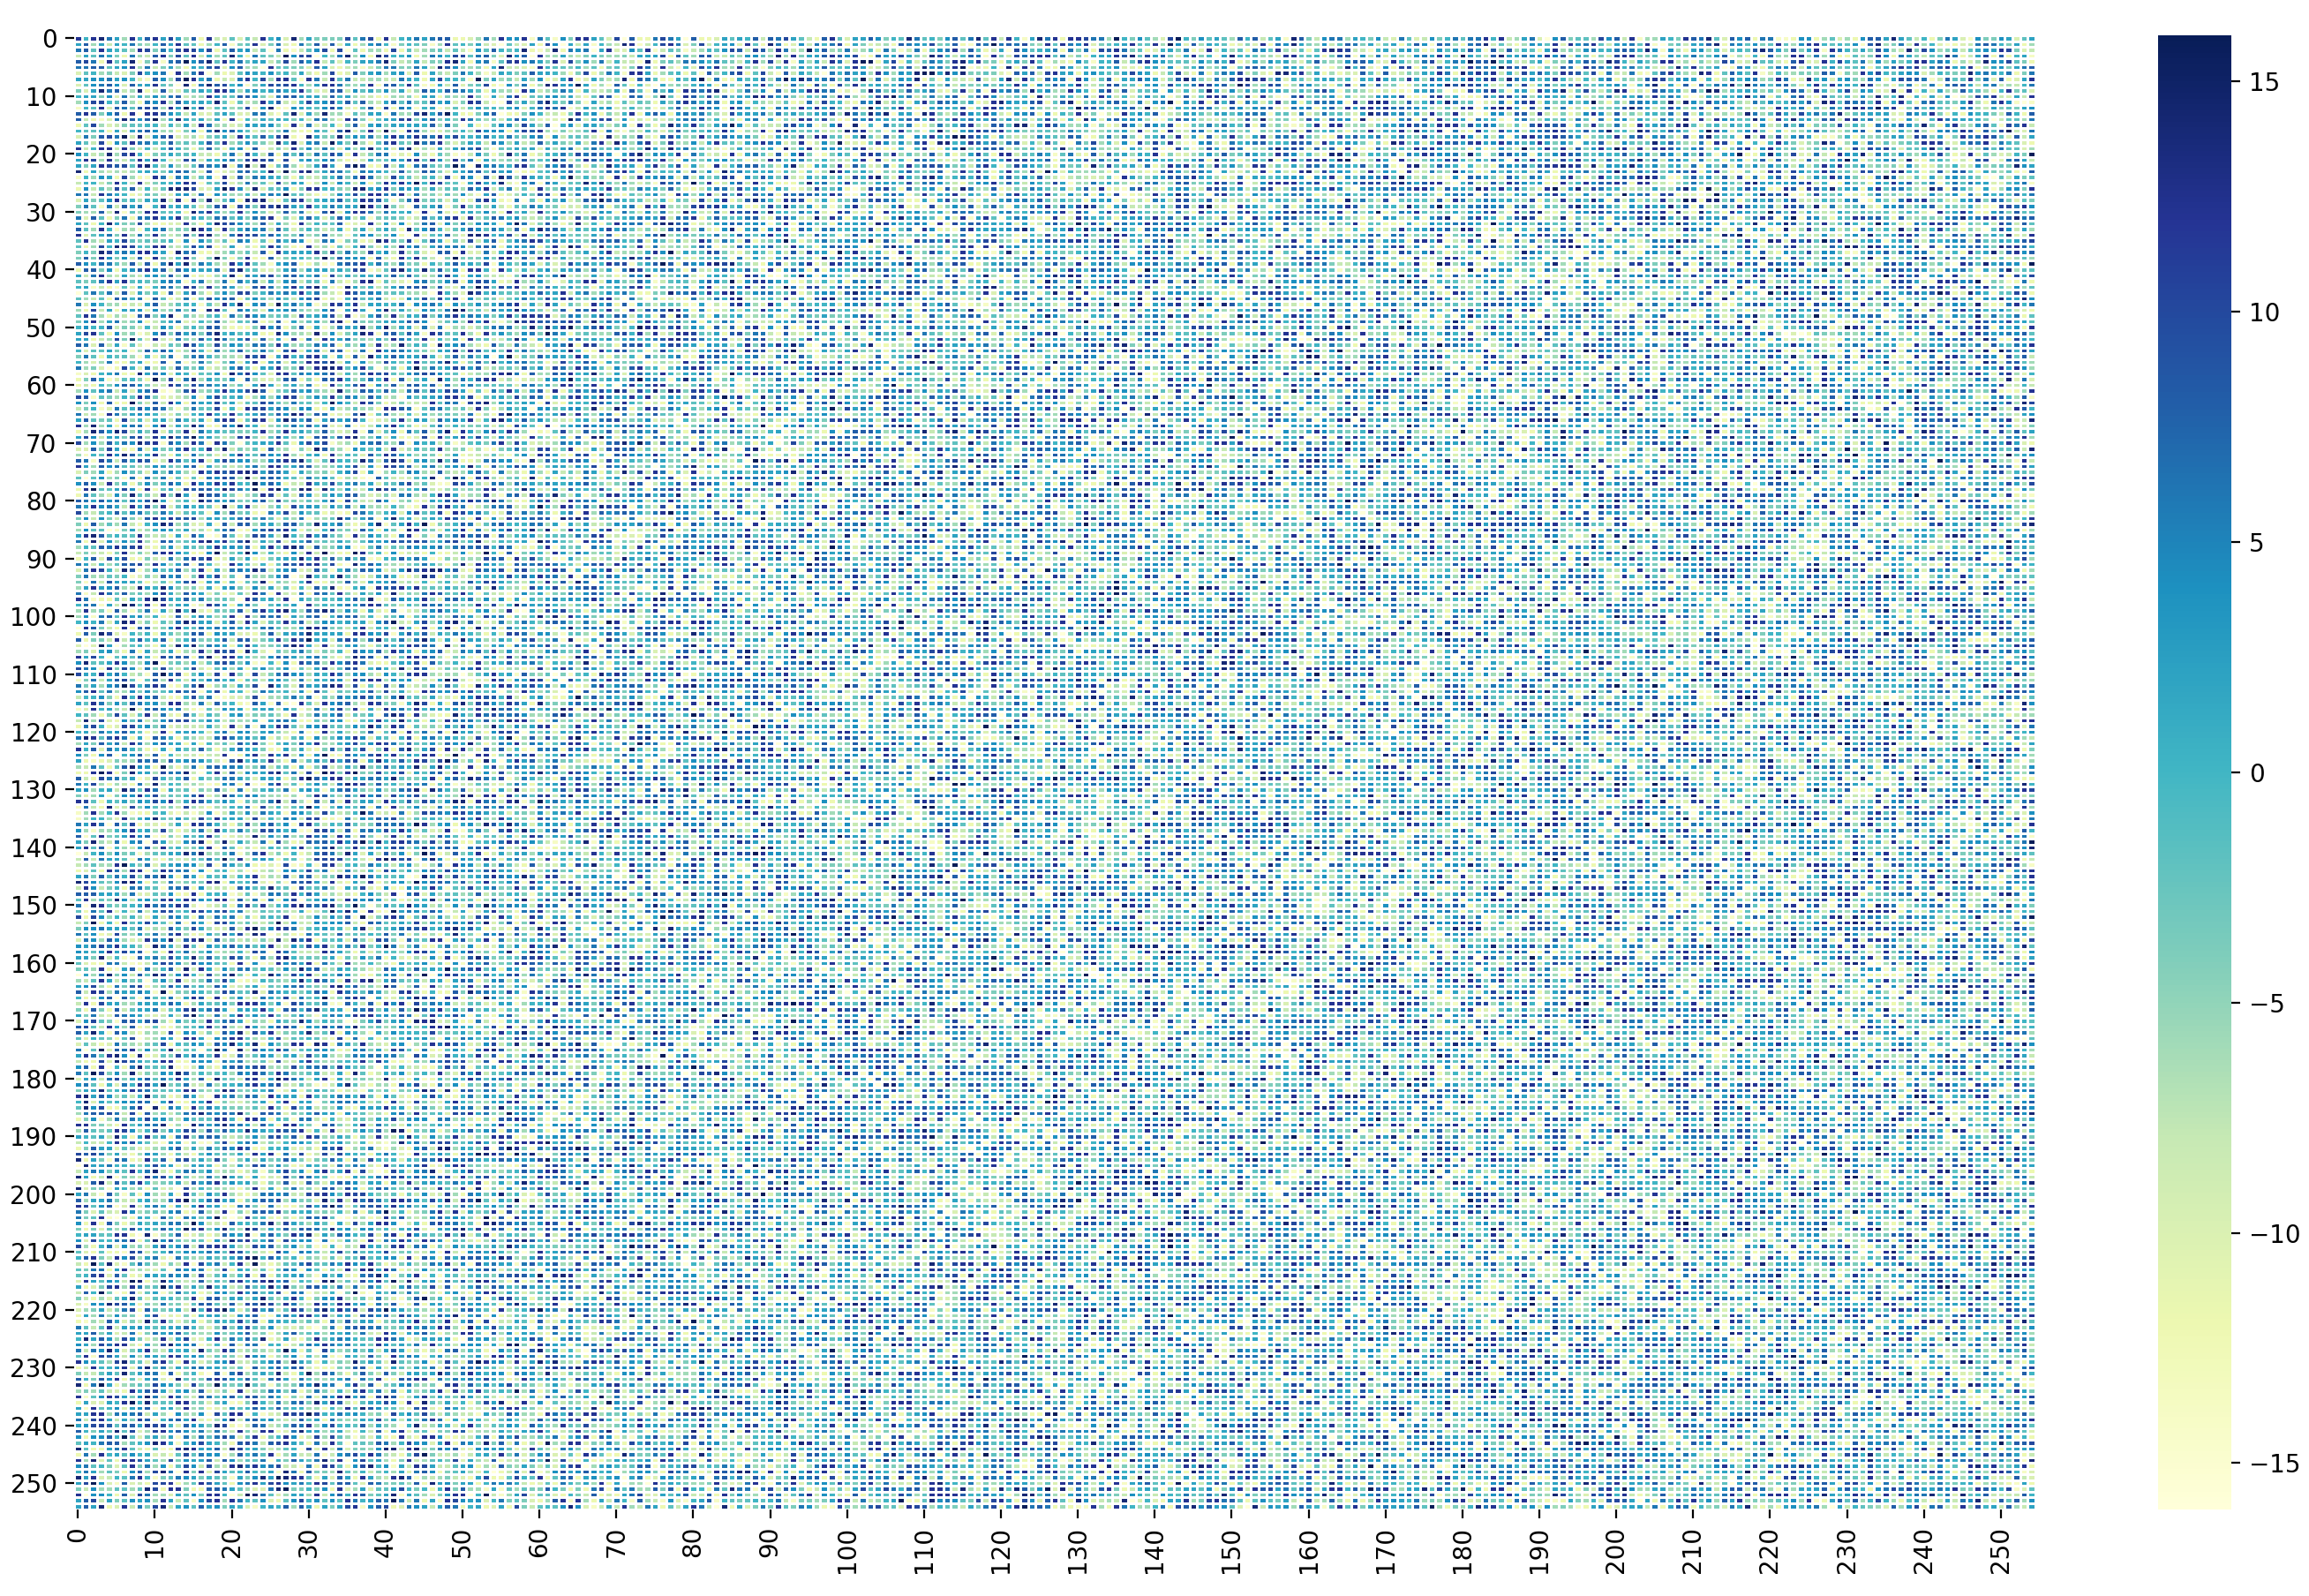
\includegraphics[scale=0.45]{lat_aes.png}
    \caption{LAT heatmap for AES $S$-Box}
    \label{fig:lat-aes}
\end{figure}

\begin{figure}
    \centering
    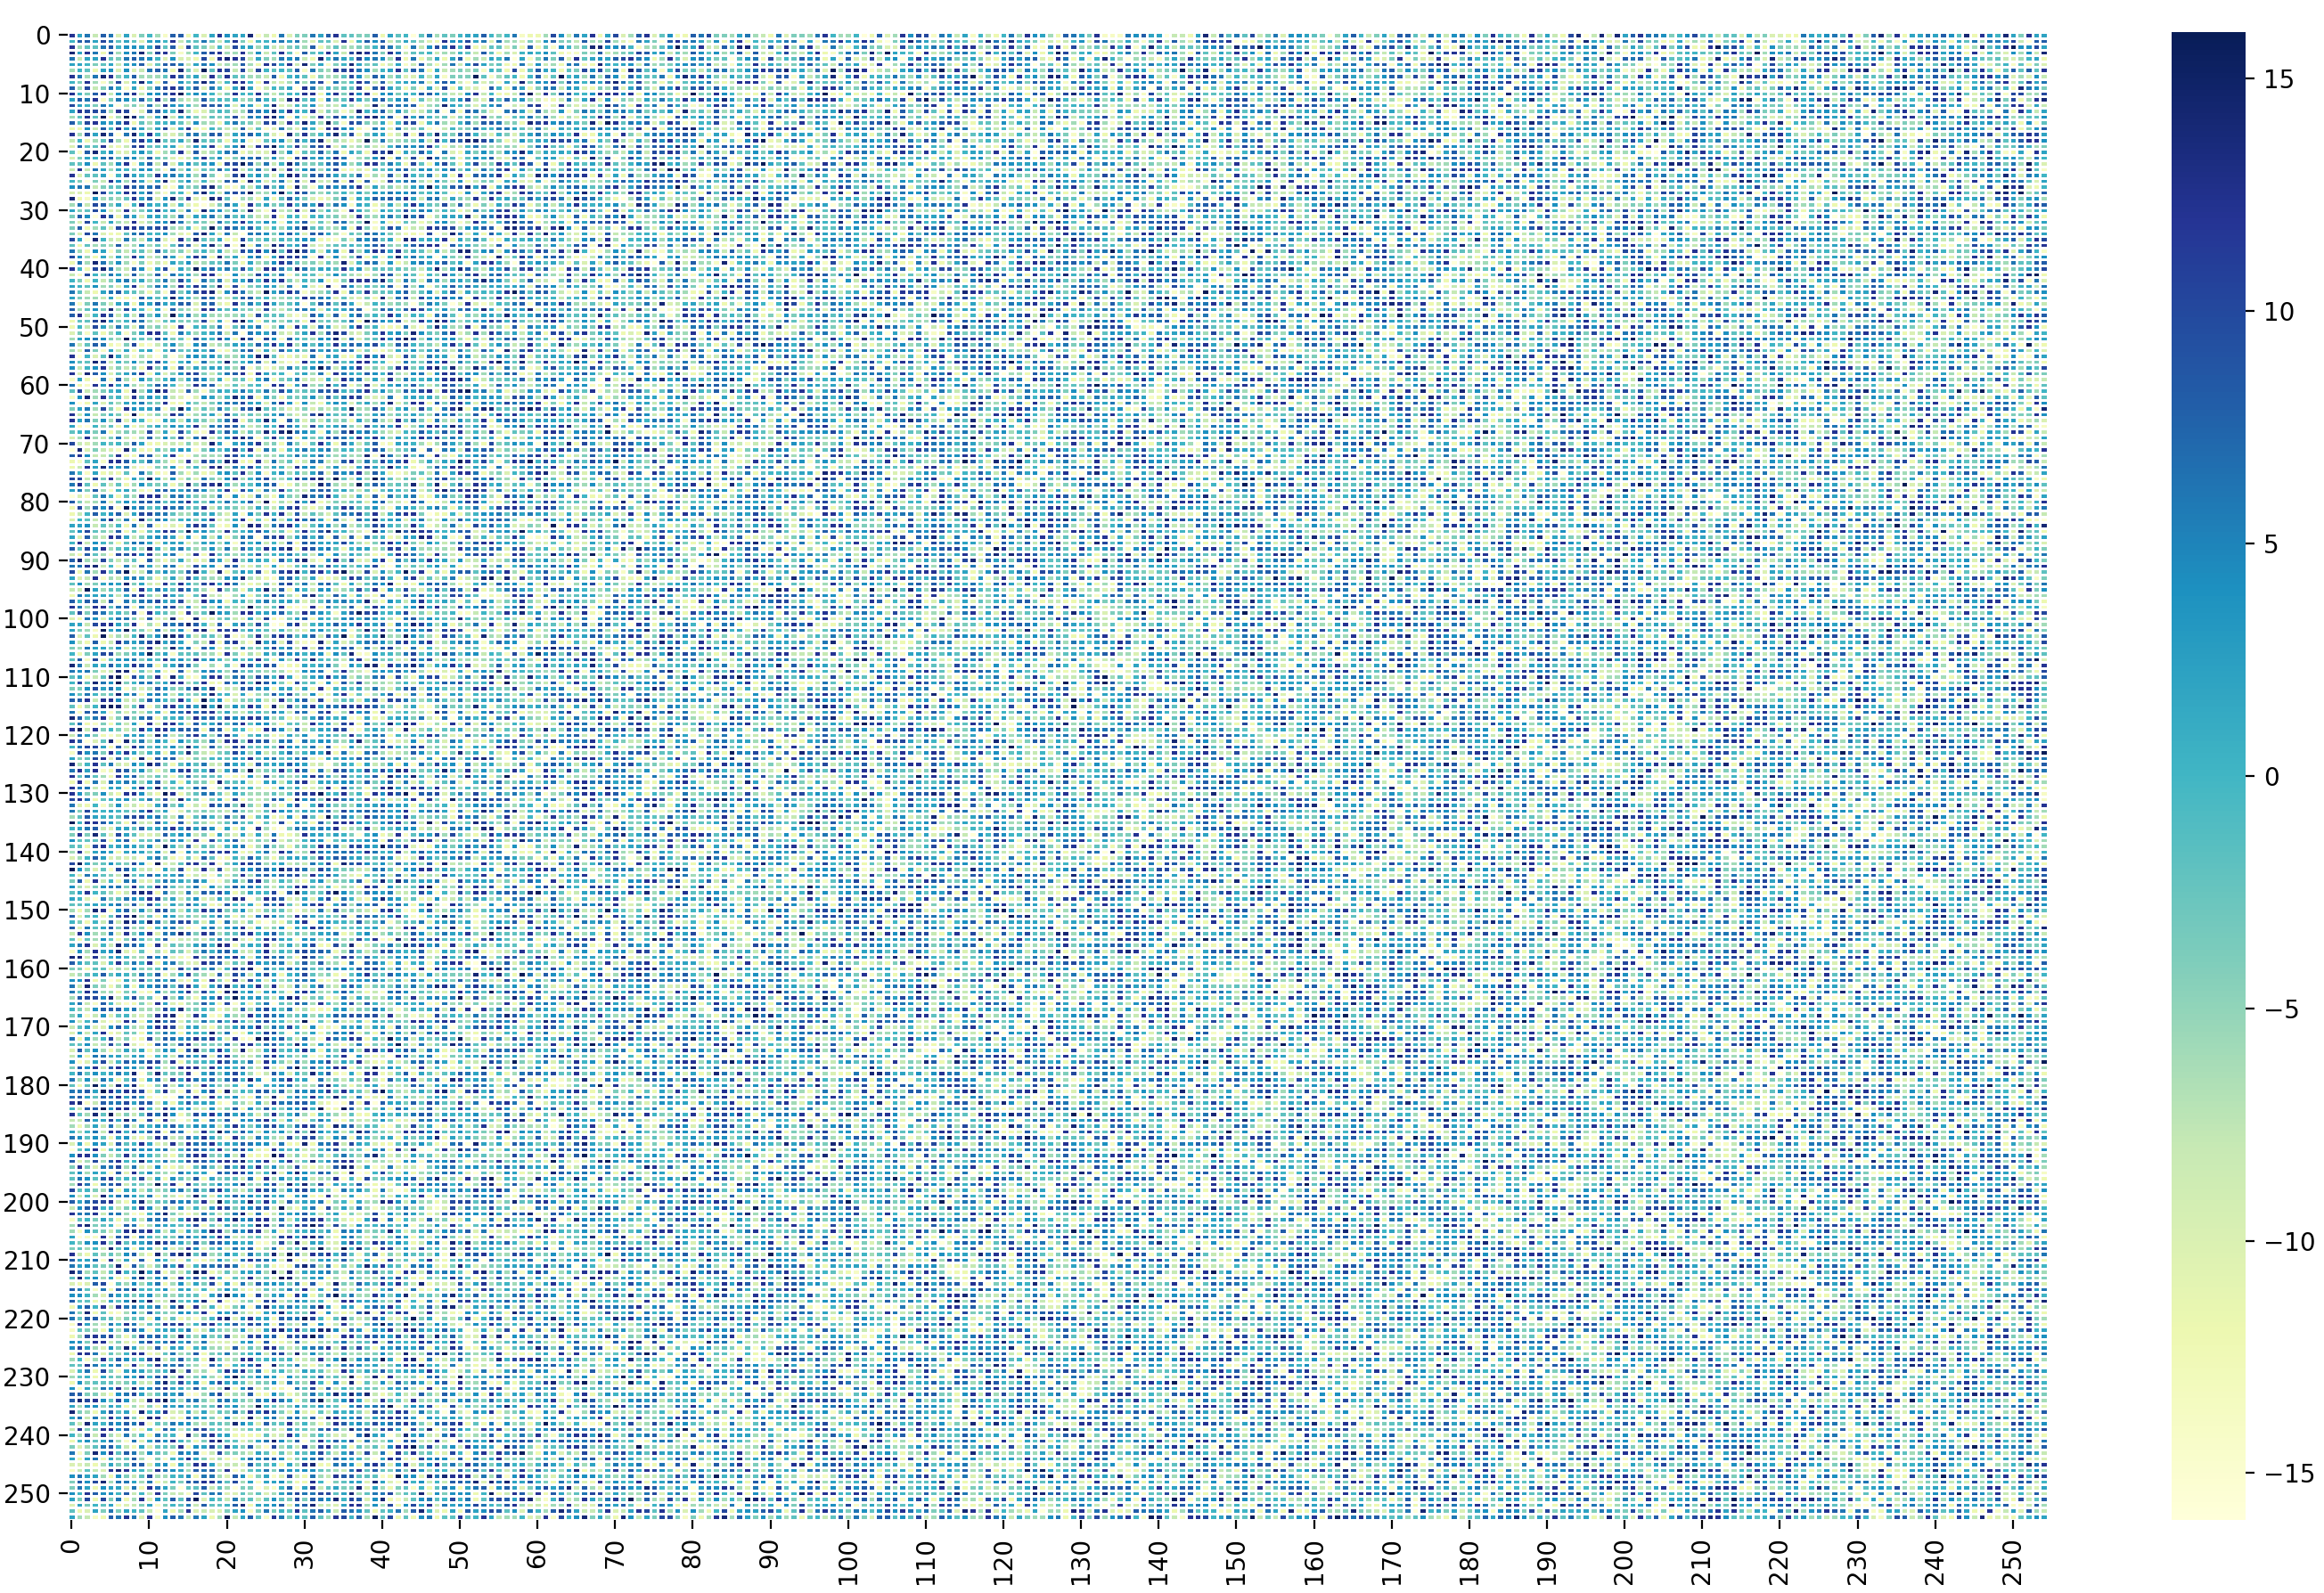
\includegraphics[scale=0.45]{lat_aes_inv.png}
    \caption{LAT heatmap for AES inverse $S$-Box}
    \label{fig:lat-aes-inv}
\end{figure}

\section{LC versus DC}
Linear Cryptanalysis is more efficient in breaking DES than Differential Cryptanalysis \cite{Shamir}, since it is capable of breaking the full 16-round DES in less steps. Furthermore, note that, in LC, we do not need \emph{joint LATs} or other means of restricting $S$-Box activation, because the usage of bit masks allows the attacker a better control of the propagation of the linear approximations. 

This suggests, as mentioned in \cite{Susan}, that the DES designers took DC in account, but not LC. Also, Matsui \cite{Matsui1993LinearCM} is able to mount an attack taking advantage of the linear uniformity, while Biham and Shamir \cite{Shamir} cannot take advantage of the differential uniformity of the DES $S$-Boxes and must find a suitable characteristic for their attack by other means, due to the difficulties incurred by the DES design against DC. See \cite{Coppersmith1994} and \textcolor{red}{Chapter X} of this work for more about DC on DES. 

Table \ref{tbl:dc-versus-lc} briefly compares the core concepts of DC and LC. Figures \ref{fig:diftrail} and \ref{fig:lintrail} show how differences (respectively linear relations) propagate through the DES $F$ function and the $S$-Boxes.

% Please add the following required packages to your document preamble:
% \usepackage{graphicx}
\begin{table}[H]
\centering
\resizebox{\textwidth}{!}{%
\begin{tabular}{c|c}
\hline
\multicolumn{1}{|c|}{\textbf{Differential Cryptanalysis Concepts}}                                                                & \multicolumn{1}{c|}{\textbf{Linear Cryptanalysis Concepts}}                                                                                                    \\ \hline
Chosen-plaintext attack (CPA)                                                                                                     & Known-plaintext attack (KPA)                                                                                                                                   \\ \hline
\begin{tabular}[c]{@{}c@{}}Invented by \\ Biham and Shamir \cite{Shamir}\end{tabular}                            & \begin{tabular}[c]{@{}c@{}}Invented by \\ Matsui \cite{Matsui1993LinearCM}\end{tabular}                                                                         \\ \hline
\begin{tabular}[c]{@{}c@{}}Difference: \\ $X' = X \oplus X^*$\end{tabular}                                                        & \begin{tabular}[c]{@{}c@{}}Bitmask: \\ $X \cdot \gamma$\end{tabular}                                                                                           \\ \hline
DDT (Difference Distribution Table)                                                                                                                               & LAT (Linear Approximation Table)                                                                                                                                                            \\ \hline
\begin{tabular}[c]{@{}c@{}}Active $S$-Box: \\ input difference $\neq 0$\end{tabular}                                              & \begin{tabular}[c]{@{}c@{}}Active $S$-Box: \\ output mask $\neq 0$\end{tabular}                                                                                \\ \hline
\begin{tabular}[c]{@{}c@{}}Distinguisher: \\ differential characteristic\end{tabular}                                             & \begin{tabular}[c]{@{}c@{}}Distinguisher: \\ linear relation (or approximation)\end{tabular}                                                                   \\ \hline
\begin{tabular}[c]{@{}c@{}}Probability of an $r$-round \\ differential characteristic: \\ $p = \prod_{i=1}^r p_i$\end{tabular}    & \begin{tabular}[c]{@{}c@{}}Bias of an $r$-round \\ linear relation: \\ $\epsilon = 2^{r-1}\cdot \prod_{i=1}^r \epsilon_i$, \\ from the Piling-up Lemma\end{tabular} \\ \hline
\begin{tabular}[c]{@{}c@{}}Chosen-plaintexts \\ for a characteristic with \\ probability $p$: \\ approximately $1/p$\end{tabular} & \begin{tabular}[c]{@{}c@{}}Known-plaintexts \\ for a linear relation with \\ bias $\epsilon$: \\ approximately $1/\epsilon^2$\end{tabular}                     \\ \hline
\begin{tabular}[c]{@{}c@{}}Differential trail \\ (follow non-zero differences)\end{tabular}                                       & \begin{tabular}[c]{@{}c@{}}Linear trail \\ (follow non-zero masks)\end{tabular}                                                                               
\end{tabular}%
}
\caption{Comparing DC and LC concepts}
\label{tbl:dc-versus-lc}
\end{table}

\begin{figure}[H]
    \centering
    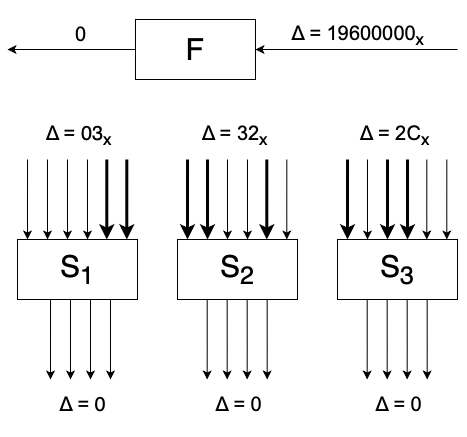
\includegraphics[scale=0.5]{Shamir-DES.png}
    \caption{Propagation of differences in DC (differential trails)}
    \label{fig:diftrail}
\end{figure}

\begin{figure}[H]
    \centering
    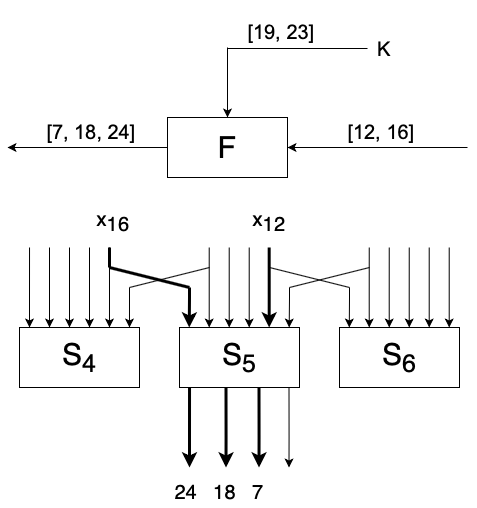
\includegraphics[scale=0.5]{Matsui-DES.png}
    \caption{Propagation of linear relations in LC (linear trails)}
    \label{fig:lintrail}
\end{figure}

\section{Conclusions}
In this chapter, we gave a brief overview of Linear Cryptanalysis and explained how to obtain LATs --- Linear Approximation Tables. We also presented LATs for DES $S$-Boxes and AES $S$-Boxes, as well as their linear uniformities. We leave the application of an actual LC attack as a future work.

\bibliographystyle{plain}
\bibliography{refs}

\end{document}
